\documentclass[10pt,utf8]{beamer}
\setbeamersize{text margin left=15pt,text margin right=15pt}
\usepackage{cmap}
\usepackage[T1,T2A]{fontenc}
\usefonttheme[onlymath]{serif}
\usepackage{paratype}
\usepackage {latexsym}
%\usepackage {fancybox}
\usepackage {fouriernc}

\usepackage{caption}
\setbeamertemplate{caption}[numbered]
%\addtobeamertemplate{navigation symbols}{}{ \hspace{1em}  \usebeamerfont{footline}  {\normalsize \insertframenumber / \inserttotalframenumber}}
\addtobeamertemplate{navigation symbols}{}{ \hspace{1em}  \usebeamerfont{footline}  {\normalsize \color{black} \insertframenumber }}

\usepackage{tikz}
% \usetikzlibrary{tikzmark,calc}
\usepackage[english,russian]{babel}
\usepackage{bropd} % od, pd

\usetheme{Warsaw}

\DeclareMathOperator*{\sign}{sign}

\usepackage{blox}
\usepackage[europeanresistors,americaninductors,siunitx,fulldiodes]{circuitikz}

\usetikzlibrary{calc}
\usetikzlibrary{arrows}
\usetikzlibrary{patterns}
%\usepgflibrary{shapes.geometric}
\usetikzlibrary{external}


\definecolor{haircolor}{rgb}{0.7,0.7,1.0}
\newcommand{\TikzAddPadding}{\path (current bounding box.north east) ++(+0.1,+0.1); \path (current bounding box.south west) ++(-0.1,-0.1);}

\tikzset{
  >=stealth,
  %semiRed/.style={fill=red,opacity=0.3,draw=black,thin},
  hair/.style={draw,color=haircolor,line width=0.1pt},
  medline/.style={draw=black,line width=0.6pt},
  medlinep/.style={draw=black,line width=0.6pt,->},
  semiboldline/.style={draw=black,line width=1.2pt},
  semiboldlinep/.style={draw=black,line width=1.2pt,->},
  infoline/.style={draw=gray,line width=1.4pt},
  boldline/.style={draw=black,line width=2.0pt},
  boldlinep/.style={draw=black,line width=2.0pt,->},
  wire/.style={draw=black,line width=1.0pt},
  elelem/.style={draw=black,line width=1.5pt},
  subelem/.style={draw=black,dashed,line width=0.6pt}
}



\newcommand{\booknameUa}{Ансамблеві пошукові моделі і методи параметричної ідентифікації систем з хаотичною поведінкою}
\newcommand{\booknameRu}{Ансамблевые поисковые модели и методы параметрической идентификации систем с хаотическим поведением}
\newcommand{\booknameEn}{Ensemble search models and methods for parametric identification of systems with chaotic behavior}
\newcommand{\bookname}{\booknameRu}

\newcommand{\bookyear}{2018}
\newcommand{\dissauthorUa}{Гуда~А.І.}
\newcommand{\dissauthorRu}{Гуда~А.И.}
\newcommand{\dissauthorEn}{Guda~A.I.}
\newcommand{\dissauthorFullRu}{Гуда Антон Игоревич}
\newcommand{\dissauthorFullUa}{Гуда Антон Ігорович}
\newcommand{\dissauthorMain}{\dissauthorRu}
\newcommand{\dissauthorAref}{\dissauthorUa}
\newcommand{\dissauthorFullMain}{\dissauthorFullRu}
\newcommand{\dissauthorFullAref}{\dissauthorFullUa}

\newcommand{\dissSpecUa}{математичне    моделювання  та обчислювальні методи}
\newcommand{\dissSpecRu}{математическое моделирование и вычислительные методы}
\newcommand{\dissSpecEn}{Mathematical Modelling and Computational Methods}
\newcommand{\dissSpecMain}{\dissSpecRu}
\newcommand{\dissSpecAref}{\dissSpecUa}
\newcommand{\dissSpecId}{01.05.02}
\newcommand{\dissScopeRu}{технических наук}
\newcommand{\dissScopeUa}{техничних наук}
\newcommand{\dissScopeMain}{\dissScopeRu}
\newcommand{\dissScopeAref}{\dissScopeUa}
\newcommand{\UDC}{004: 681.5.015}
\newcommand{\dissRada}{Д.~08.084.01}
\newcommand{\dissSekrRadi}{Селівьорстова~Т.В.}
\newcommand{\institutionRu}{Национальная металлургическая академия Украины}
\newcommand{\institutionUa}{Національна  металургійна     академія України}
\newcommand{\institutionEn}{National Metallurgical academy of Ukraine}
\newcommand{\institutionMain}{\institutionRu}
\newcommand{\institutionAref}{\institutionUa}
\newcommand{\belongRu}{Министерство образования и науки Украины}
\newcommand{\belongUa}{Міністерство освіти і науки      України}
\newcommand{\belongEn}{Ministry of Education and Science of Ukraine}
\newcommand{\belongMain}{\belongRu}
\newcommand{\belongAref}{\belongUa}
\newcommand{\cityRu}{Днепр}
\newcommand{\cityUa}{Дніпро}
\newcommand{\cityEn}{Dnipro}
\newcommand{\cityMain}{\cityRu}
\newcommand{\cityAref}{\cityUa}
\newcommand{\superRu}{Михалёв Александр Ильич}
\newcommand{\superUa}{Михальов Олександр Ілліч}
\newcommand{\superMain}{\superRu}
\newcommand{\superAref}{\superUa}



\author{\dissauthorRu}

\title[Семинар -- 2017]{\booknameRu}

\newlength\TW
\setlength{\TW}{0.01\textwidth} % after geometry!
\newlength\DDW
\setlength{\DDW}{0.36\textwidth}

\begin{document}

\begin{frame}
  \frametitle{}
  \begin{center}
    {\Large \color{blue} \booknameRu}

    \vfill

    {\large \dissauthorMain}

    \vfill

    Научный консультант -- д.т.н., проф. \superRu

    \vfill

    Днепр -- 2017
  \end{center}
\end{frame}

% -----------------------------------------------------------------------

\begin{frame}
  \frametitle{Актуальность}
  %\framesubtitle{}

  Актуальность обусловлена следующими фактами:

  \begin{itemize}

    \item
      Нелинейные динамические системы, представленные в современных
      технологических процессах, природных явлениях, зачастую
      демонстрируют хаотическое поведение.
      Основная причина -- малые возмущения параметров или входных сигналов
      приводят к существенным изменениям выходного сигнала.

    \item
      Существующие методы идентификации или принципиально непригодны для
      работы с хаотическими системами, или же требуют выполнения
      достаточно жёстких условий.

    \item
      Существуют динамические системы, не обладающие строгими свойствами хаотичности,
      но имеющие с ними общие свойства с точки зрения идентификации.

    \item
      Свойства существующих методов идентификации нелинейных динамических систем
      ограничивают достижимое качество идентификации,
      особенно применительно к хаотическим системам.

  \end{itemize}


\end{frame}


% -----------------------------------------------------------------------

\begin{frame}
  \frametitle{Объект, предмет, методы}
  %\framesubtitle{}

\textbf{Объект исследования} ---
технические системы, которые в процессе функционирования
могут входить в хаотический режим.

\medskip

\textbf{Предмет исследования} ---
математические модели процессов и методы
адаптивно-поисковой идентификации технических систем с хаотической динамикой.

\medskip

\textbf{Методы исследования} ---
математический аппарат теории управления и идентификации,
динамического хаоса,
нечёткой логики,
теории информации,
вычислительные методы
\ldots

\end{frame}



% -----------------------------------------------------------------------

\begin{frame}
  \frametitle{Задачи исследования}
  %\framesubtitle{}

  \begin{itemize}

    \item
      Разработать новые критерии идентификации, которые, в отличие от существующих,
      при моделировании были бы пригодны для анализа состояния и динамики хаотических
      систем, что создаст основу для создания работоспособных систем идентификации.

    \item
      Развить существующие и разработать новые методы поиска, которые в полной мере
      использовали преимущества использования ансамбля поисковых агентов.

    \item
      Разработать новые и развить существующие и  методы настройки параметров системы
      идентификации, способные приспособиться к смене режимов работы системы.

    \item
      Разработать программное обеспечение, пригодное для моделирования как систем
      хаотической динамики, так и систем идентификации.

    \item
      Провести компьютерное моделирование процессов идентификации систем хаотической
      динамики и исследовать их работоспособность, возможности и характеристики.

  \end{itemize}

\end{frame}



% -----------------------------------------------------------------------

\begin{frame}
  \frametitle{Прототипы}
  %\framesubtitle{}

  Кто занимался и какие методы.


\end{frame}







% -------------------------- P2 ---------------------------------------------


% -----------------------------------------------------------------------

\begin{frame}
  \frametitle{Необходимость новых критериев}
  \framesubtitle{Влияние малых возмущений}


\end{frame}



% -----------------------------------------------------------------------

\begin{frame}
  \frametitle{Определения идентификации}
  %\framesubtitle{}

  Заде -- Райбман, \ldots


\end{frame}

% -----------------------------------------------------------------------


\begin{frame}
  \frametitle{Критерии идентификации: требования}
  %\framesubtitle{}


\end{frame}



% -----------------------------------------------------------------------

\begin{frame}
  \frametitle{Критерии идентификации: энергетические основы}
  %\framesubtitle{}


\end{frame}



% -----------------------------------------------------------------------

\begin{frame}
  \frametitle{Критерии идентификации: предлагаемый набор величин}
  %\framesubtitle{}


\end{frame}



% -----------------------------------------------------------------------

\begin{frame}
  \frametitle{Отличие задачи идентификации}
  %\framesubtitle{}


\end{frame}



% -----------------------------------------------------------------------

\begin{frame}
  \frametitle{Динамические характеристики критериев}
  %\framesubtitle{}


\end{frame}



% -----------------------------------------------------------------------

\begin{frame}
  \frametitle{Выводы?}
  %\framesubtitle{}


\end{frame}



% --------------------------- P3 --------------------------------------------



\begin{frame}[fragile]
  \frametitle{Безразмерный вид критерия и функции качества}
  %\framesubtitle{}

  Критерий, основанных на физических принципах -- чаще всего размерная величина.
  Используются 2 способа обезразмеривания: деление
  на какую-либо характерную величину той же размерности,
  использование функции качества.

  \begin{tabular}{p{45\TW}|p{52\TW}}
  \[
      q_r = \frac{q_o - q_m}{q_\gamma},
  \]
  \begin{equation}
    F_{\mathrm{gauss}} = \exp( - q_r^2 ),
  \label{atu:eq:F_gauss}
  \end{equation}
  %
  \begin{equation}
    F_{\mathrm{parabolic}} = 1 - q_r^2 \left( 1 - \frac{1}{e} \right),
  \label{atu:eq:F_parabolic}
  \end{equation}
  %
  \begin{equation}
    F_{\mathrm{triangle}} = 1 - |q_r| \left( 1 - \frac{1}{e} \right),
  \label{atu:eq:F_triangle}
  \end{equation}
  %
  \begin{equation}
    F_{\mathrm{hyper}} = \frac{1}{ 1 + |q_r| \left( 1 - \frac{1}{e} \right)},
  \label{atu:eq:F_hyper}
  \end{equation}
  %
  \begin{equation}
    F_{\mathrm{log}} = 1 - \ln \left( 1 + |q_r| \right) \frac{1-1/e}{\ln(2)}.
  \label{atu:eq:F_log}
  \end{equation}
 &
  \begin{figure}[htb!]
    \centerline{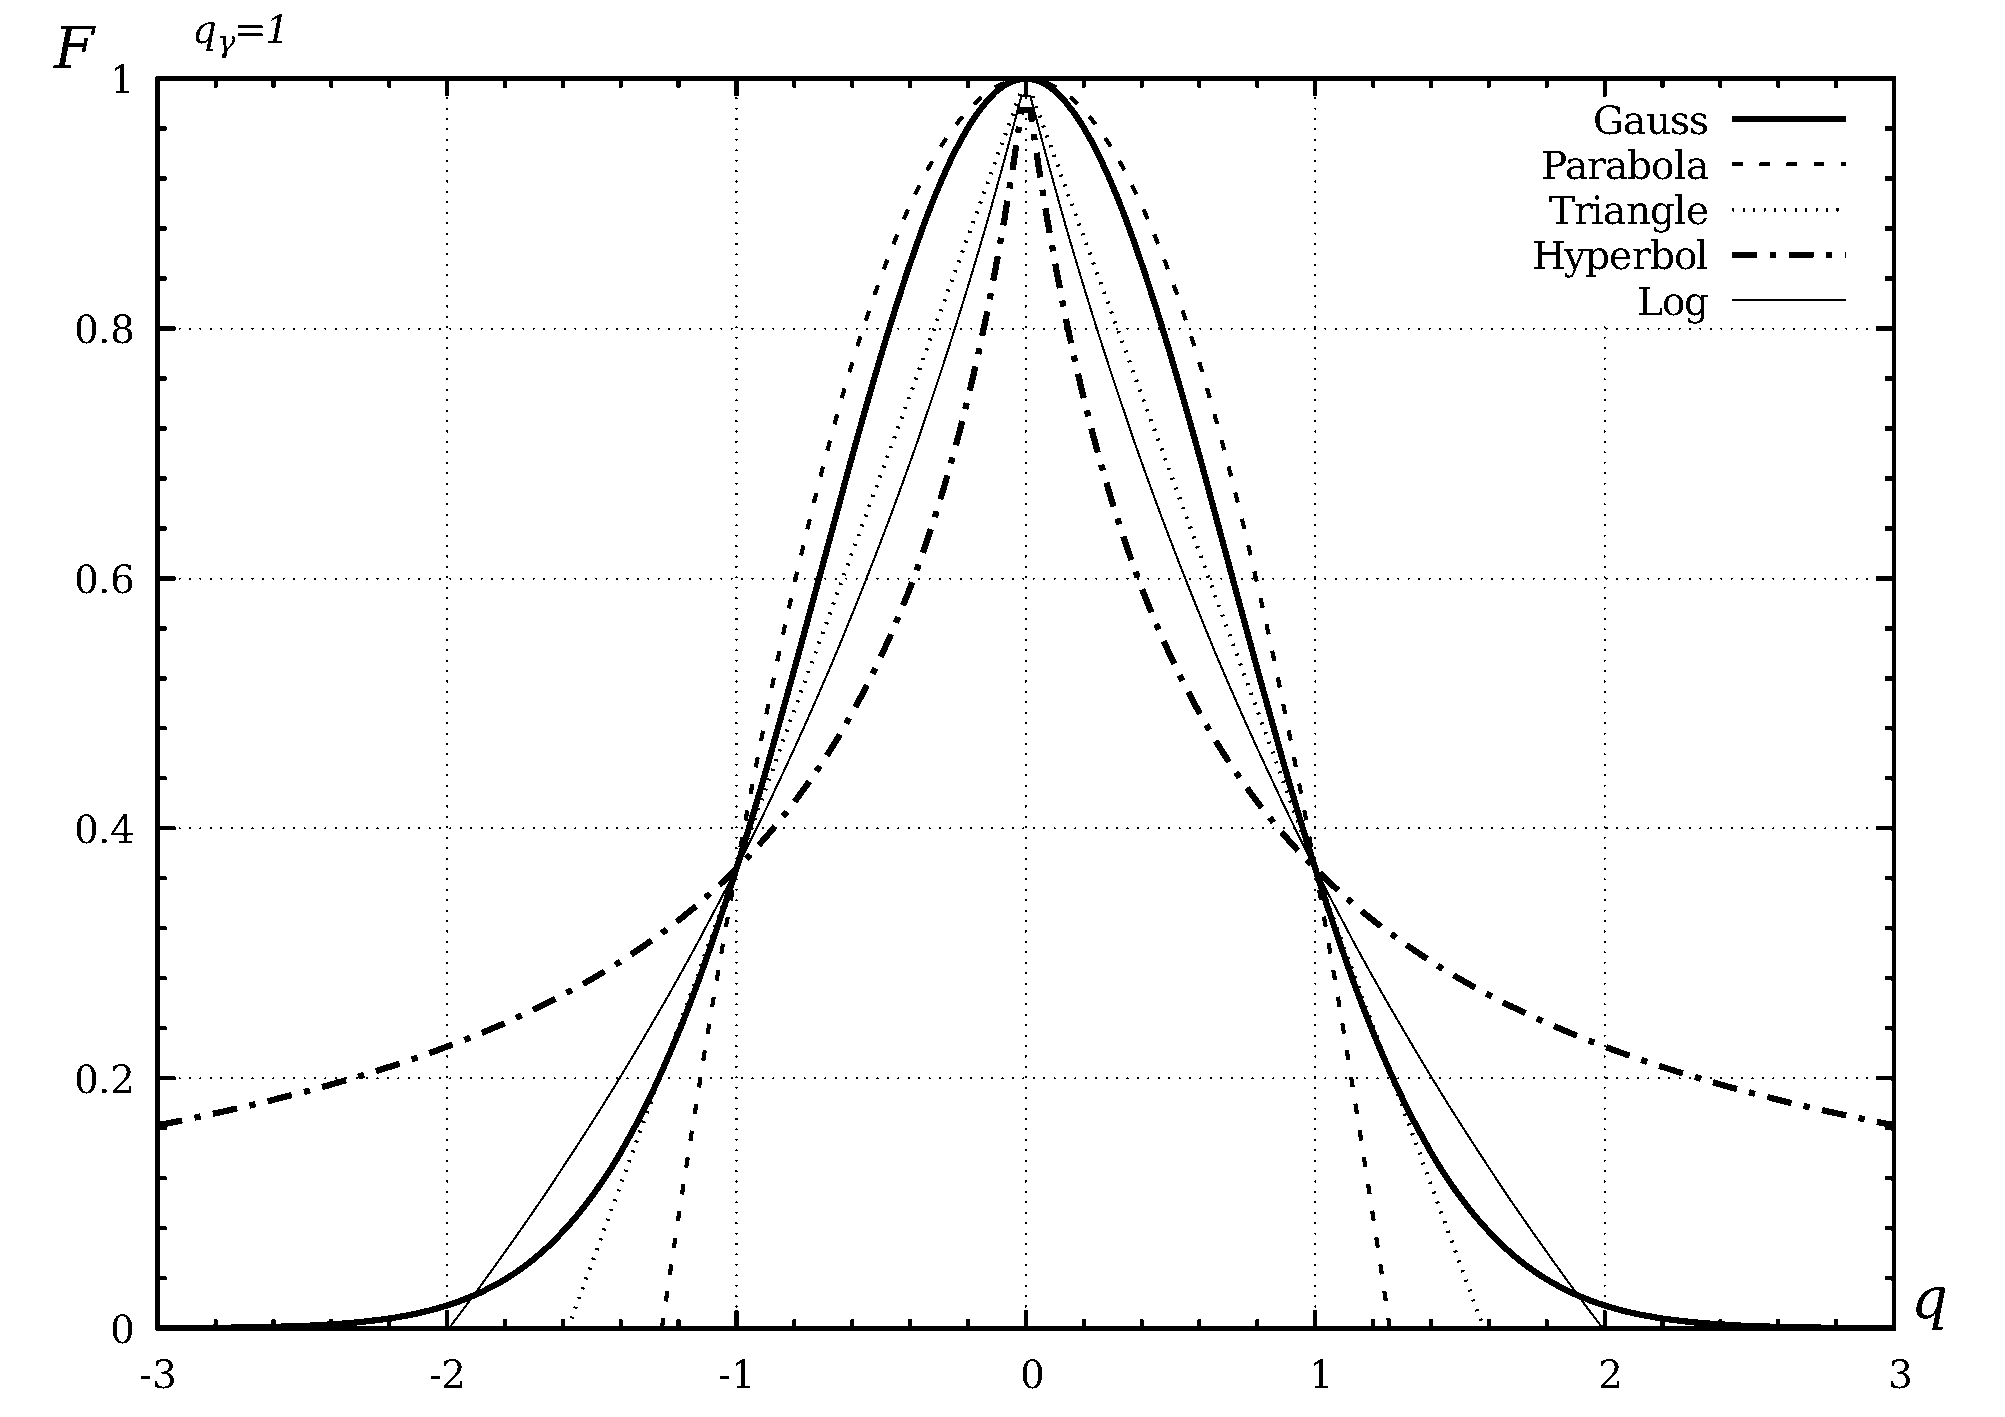
\includegraphics[width=0.45\textwidth]{p/F_types.png} }
    \caption{Функции качества идентификации (\ref{atu:eq:F_gauss})--(\ref{atu:eq:F_log})}
    \label{atu:f:F_types}
  \end{figure}
  \end{tabular}



\end{frame}

% -----------------------------------------------------------------------


\begin{frame}
  \frametitle{Элементы системы идентификации: определения}
  %\framesubtitle{}

  Определение: \textbf{поисковый агент} -- это динамическая система, получающая выходной ($x(t)$),
  и, при необходимости входной сигнал ($u(t)$) от одной или нескольких моделей,
  величину оцкнци состояния объекта по критерию идентификации $q_o(t)$,
  может быть обмениваясь информацией с другими элементами поисковой системы,
  на основании значения критерия идентификации
  реализующая алгоритм настройки параметра модели (моделей)
  таким образом, чтобы обеспечить идентификацию заданного параметра.

  Определение: \textbf{координатор поиска} -- это динамическая система, получающая информацию
  от поисковых агентов, и на основании этой информации определяющая
  $p_{\mathrm{id}}(t)$ -- искомую величину идентифицируемого параметра.
  Помимо этого, координатор может, на основании этой же информации,
  управлять процессом адаптации всей поисковой системы.

\end{frame}



% -----------------------------------------------------------------------

\begin{frame}[fragile]
  \frametitle{Плоская структура мультиагентной системы}
  %\framesubtitle{}

  \begin{figure}[ht!]
  \begin{center}
  ../../p3/p/agents.pgf
  \end{center}
  \caption{Мультиагентная система идентификации с плоской структурой}
  \label{atu:f:agents_flat}
  \end{figure}

\end{frame}



% -----------------------------------------------------------------------

\begin{frame}
  \frametitle{Виды мультиагентных систем идентификации}
  %\framesubtitle{}

  \begin{description}
    \item[Рой]
      --- множество агентов, обеспечивающее идентификацию за счёт
      сосредоточения максимального количества агентов
      в области предполагаемого максимума функции качества или же
      заданного значения критерия.
      Обычно -- три составляющие поведения
      (движение о оцениваемому локальному экстремуму, -- к глобальному, случайная составляющая).

    \item[Строй]
      --- множество агентов, расположение которых,
      и если необходимо, смещение, задаётся
      единообразным образом.
      Отсутствует индивидуальная динамика каждого агента.
      Неподвижный строй образует \textbf{сетку},
      как равномерно распределённую по пространству параметров,
      так и нет.

    \item[Ансамбль]
      --- множество агентов, обеспечивающее идентификацию за счёт
      распределения агентов таким образом, который обеспечивает как
      точность идентификации за счёт ограниченного скопления агентов
      в областях предполагаемых максимумов, так и оперативное переключение
      на другие области при изменении параметров за счёт недопущения
      неоправданной скученности агентов.
   \end{description}

\end{frame}



% -----------------------------------------------------------------------

\begin{frame}
  \frametitle{Виды и задачи поисковых агентов}
  %\framesubtitle{}

  Один поисковый агент может управлять как одной моделью (рис.~\ref{atu:f:agent1}, \ref{atu:f:agent1q}),
  так и несколькими (рис.~\ref{atu:f:agent2}).
  При этом он может использовать информацию,
  как полученную непосредственно от других агентов,
  так и вычисленную в результате обработки данных на других уровнях системы идентификации.

  Группировки агентов: пары (``l'', ``r''), триплеты (``l'', ``c'', ``r'').
  Группы могут быть независимы или же пересекаться.


  Выходные сигналы агента: \\
  $p_c(t)$ --- текущее значение параметра (центр), \\
  $F_c(t)$ --- значение функции качества, \\
  $q_c(t)$ --- значение критерия качества, \\
  $p_e(t)$ --- оценка идентифицируемого параметра текущим агентом, \\
  $S_e(t)$ --- степень ``уверенности'' агента в полученном значении.

\end{frame}



% -----------------------------------------------------------------------

\begin{frame}
  \frametitle{Один агент --- несколько моделей}
  %\framesubtitle{}


  \begin{figure}[htb!]
    \begin{center}
      % vi:syntax=tex
\begin{tikzpicture}
  %\draw[hair,step=1.0em] (0,-3) grid (12.0,3.0);
  \bXStyleBloc{semiboldline,inner sep=2pt};
  \bXLineStyle{medline};
  % --- U
  \bXInput{U};
  \path (U.center) ++(2.5em,0.0em) coordinate (UxM);
  \draw (U.center) -- (UxM);
  \fill (UxM) circle[radius=0.05];
  \node[above right] at(U) {$u(t)$};
  % --- M0
  \bXBranchy[2]{UxM}{U0};
  %\fill[red](U0) circle[radius=0.05];
  \bXBlocL[2.0]{M0}{$\mathbf{M}_{i0}$}{U0};
  \bXLinkyx{UxM}{M0};
  % --- M1
  \bXBranchy[-2]{UxM}{U1};
  %\fill[green](U1) circle[radius=0.05];
  \bXBlocL[2.0]{M1}{$\mathbf{M}_{i1}$}{U1};
  \bXLinkyx{UxM}{M1};
  % --- A
  \path (M0.east) ++(3.1em,0.0em) coordinate (X0);
  \path (X0) ++(4.0em,0.0em) coordinate (P0S);
  \path (X0) ++(0.0em,-2.0em) coordinate (Alb);
  %\fill[red](Alb) circle[radius=0.05];
  \path (M1.east) ++(3.1em,0.0em) coordinate (X1);
  \path (X1) ++(4.0em,0.0em) coordinate (P1S);
  \path (X1) ++(0.0em,2.0em) coordinate (Alt);
  \path ( $0.5*(P0S) + 0.5*(P1S)$ ) coordinate(PS);
  \path ( $0.5*(X0) + 0.5*(X1)$ ) coordinate(QO);
  \draw[medlinep] (QO) ++(-3.2em,0em) -- (QO);
  \node[above left] at(QO) {$q_{o}(t)$};
  %\fill[green](Alt) circle[radius=0.05];
  \draw[boldline] (Alb) -- ++(4.0em,0.0em) |- (Alt) -- cycle; % ----- MAIN block
  \draw[medlinep] (M0.east) -- (X0); // % inputs: x_ix(t)
  \node[above right] at(M0.east) {$x_{i0}(t)$};
  \draw[medlinep] (M1.east) -- (X1);
  \node[above right] at(M1.east) {$x_{i1}(t)$};
  \draw[semiboldlinep] (P0S) -- ++(3.0em,0em) -- ++(0em,-3.0em) -| (M0.south); % -- out params
  \node[above right] at(P0S) {$p_{i0}(t)$};
  \draw[semiboldlinep] (P1S) -- ++(3.0em,0em) -- ++(0em,+3.0em) -| (M1.north);
  \node[above right] at(P1S) {$p_{i1}(t)$};
  \draw[medlinep] (PS) -- ++(4.0em,0em);
  \node[above right] at(PS) {$p_{i}(t)$};
  \path (PS) ++(-2.1em,0.0em) coordinate (AI);
  \node at(AI) {$\mathbf{A}_{i}$};
  %
  \TikzAddPadding
  %
\end{tikzpicture}

    \end{center}
    \caption{Поисковый агент, настраивающий параметры двух моделей}
    \label{atu:f:agent2}
  \end{figure}


\end{frame}



% -----------------------------------------------------------------------

\begin{frame}
  \frametitle{Методы агентов, использующих значения критерия}
  %\framesubtitle{}

  \begin{figure}[htb!]
  \begin{center}
  % vi:syntax=tex
\begin{tikzpicture}
  \bXStyleBloc{semiboldline,inner sep=2pt};
  \bXLineStyle{medline};
  % --- U
  \bXInput{U};
  % --- M
  \bXBlocL[2.0]{M}{$\mathbf{M}_i$}{U};
  \bXLink[$u(t)$]{U}{M};
  % --- Q
  \bXBloc[3.5]{Q}{$q$}{M};
  \path (Q.east) ++(0.0,-1.0em) coordinate (Qqm);
  \path (Q.south west) ++(-0.3,-0.4) coordinate (BLKlb);
  \bXLink[$x_i(t)$]{M}{Q};
  % --- P
  \bXBloc[2]{P}{$P$}{Q};
  \draw[infoline,<->] (P.north) -- +(0,0.8);
  \path (P.west) ++(0.0,-1.0em) coordinate (Pqm);
  \path (P.west) ++(0.0,+1.0em) coordinate (Pqo);
  \path (Pqo) ++(-1.6em,+2.8em) coordinate (Pqoi) {};  % external input
  \path (P.north east) ++(0.1,+0.4) node (BLKrt) {};
  \bXLink[$q_{i}(t)$]{Qqm}{Pqm};
  \draw[medlinep] (Pqoi) |- (Pqo);
  \node[below right] at (Pqoi) {$q_o(t) \qquad A_i$};
  %\bXLink[$F_i(t)$]{F}{P};
  % -- output
  \bXOutput[2.8]{Po}{P};
  \bXLink[$p_i(t)$]{P}{Po};
  \bXOutput[1.0]{Por}{P};
  \fill(Por) circle[radius=0.05];
  \bXLineStyle{semiboldline};
  \bXReturn{Por}{M}{$p_i(t)$};
  % -- block
  \draw[subelem] (BLKlb) |- (BLKrt) |- (BLKlb);
  \bXStyleBlocDefault;
  \bXDefaultLineStyle;
  %
  \TikzAddPadding
  %
\end{tikzpicture}

  \end{center}
  \caption{Поисковый агент, использующий критерий $q$, и настраивающий параметр одной модели}
  \label{atu:f:agent1q}
  \end{figure}


\end{frame}


% -----------------------------------------------------------------------

\begin{frame}
  \frametitle{Методы агентов, использующих значения функции качества}
  %\framesubtitle{}

  \begin{figure}[htb!]
  \begin{center}
  % vi:syntax=tex
\begin{tikzpicture}
  \bXStyleBloc{semiboldline,inner sep=2pt};
  \bXLineStyle{medline};
  % --- U
  \bXInput{U};
  % --- M
  \bXBlocL[2.0]{M}{$\mathbf{M}_i$}{U};
  \bXLink[$u(t)$]{U}{M};
  % --- Q
  \bXBloc[3.5]{Q}{$q(t)$}{M};
  \path (Q.east) ++(0.0,-1.0em) coordinate (Qqm);
  \path (Q.south west) ++(-0.3,-0.4) coordinate (BLKlb);
  \bXLink[$x_i(t)$]{M}{Q};
  % --- F
  \bXBloc[2.5]{F}{$F(q_o,q_{mi})$}{Q};
  \path (F.west) ++(0.0,-1.0em) coordinate (Fqm);
  \path (F.west) ++(0.0,+1.0em) coordinate (Fqo);
  \path (Fqo) ++(-1.6em,+2.8em) coordinate (Fqoi) {};  % external input
  \draw[medlinep] (Fqoi) |- (Fqo);
  \node[below right] at (Fqoi) {$q_o(t)$};
  \bXLink[$q_i(t)$]{Qqm}{Fqm};
  % --- P
  \bXBloc[2]{P}{$P$}{F};
  \draw[boldline,<->] (P.north) -- +(0,0.8);
  \path (P.north east) ++(0.1,+0.4) node (BLKrt) {};
  \bXLink[$F_i(t)$]{F}{P};
  % -- output
  \bXOutput[2.8]{Po}{P};
  \bXLink[$p_i(t)$]{P}{Po};
  \bXOutput[1.0]{Por}{P};
  \fill(Por) circle[radius=0.05];
  \bXLineStyle{semiboldline};
  \bXReturn{Por}{M}{$p_i(t)$};
  % -- block
  \draw[subelem] (BLKlb) |- (BLKrt) |- (BLKlb);
  \bXStyleBlocDefault;
  \bXDefaultLineStyle;
  %
  \TikzAddPadding
  %
\end{tikzpicture}

  \end{center}
  \caption{Поисковый агент, использующий функцию качества $F$, и настраивающий параметр одной модели}
  \label{atu:f:agent1}
  \end{figure}


\end{frame}




% -----------------------------------------------------------------------

\begin{frame}
  \frametitle{Методы, параметры и алгоритмы работы поисковых координаторов }
  %\framesubtitle{}


\end{frame}



% -----------------------------------------------------------------------

\begin{frame}
  \frametitle{Классификация и обозначения систем идентификации}
  %\framesubtitle{}

  \begin{center}
    \textbf{[qFx][bglex][clsu][zvbs][ntdsr]N.M[zra].\{crit\}}
  \end{center}

  Первый символ --- какая величина используется агентом для определения $p_e$.
  Второй --- способ определения $p_\mathrm{id}$ по всем агентам.
  Третий --- зависимость $f_e(p_e)$.
  Четвёртый --- как $f_t$ (или её эквивалент) влияет на динамику агента.
  Пятый --- поисковое движение.
  N --- количество и конфигурация агентов.
  M --- количество агентов в группе.
  [zra] --- вид модели на границе.
  \{crit\} --- критерий.

  \textbf{``Fglv5.3z.$q_{x^2}$''} -- Метод, использующий 5 подвижных (3 триплета) и 2 ``fake'' модели,
  ``global COG'' для результирующего значения параметра
  для оценивания величины $p_e$ используется функция качества,
  зависимость $f_e$ от $p_e$ -- линейная, ``вязкая'' динамика, критерий ``$q_{x^2}$''.

  \textbf{``xblst1''} -- Оригинальный адаптивно-поисковый метод.

  \textbf{``xblvd1.2''} -- Адаптивно-поисковый метод с двумя моделями и двумя УГПК с общим сбросом
    и непосредственным использованием выходов объекта и моделей.

  \textbf{``Fblvd1.2.$q_{x^2}$''} -- Адаптивно-поисковый метод с двумя моделями и двумя УГПК с общим сбросом,
   использующий функцию качества применительно к критерию $q_{x^2}$.
\end{frame}




% -----------------------------------------------------------------------

\begin{frame}
  \frametitle{Ошибки и качество идентификации}
  %\framesubtitle{}

  Два подхода --- по критерию и по ошибке идентификации $e(t)=p_o(t)-p_\mathrm{id}(t)$.
  %
  \[
    \overline{e} = \mu( p_o(t), p_\mathrm{id}(t) ),
    \quad
    t \in [0;T].
  \]
  %
  \begin{equation}
    \overline{e_c}(p_o(t),p_\mathrm{id}(t))
    =
    \max \big| p_o(t)-p_\mathrm{id}(t) \big|,
    \quad
    t \in [0;T].
    \label{atu:eq:e_c}
  \end{equation}
  %
  \begin{equation}
    \overline{e_2}(p_o(t),p_\mathrm{id}(t))
    =
    \sqrt{ \frac{1}{T} \int\limits_{0}^{T} \big( p_o(t)-p_\mathrm{id}(t) \big)^2 \, \mathrm{d}t },
    \label{atu:eq:e_2}
  \end{equation}

  Нормированные величины ошибок ( $p_{00}$ -- центр $\mathcal{P}$
  $ \overline{e}_{00}  = \overline{e}(p_o(t),p_{00})$ ):
  %
  \begin{equation}
    \overline{e}_{rge} = \frac{\overline{e}_{ge}}{\overline{e}_{00}}, \;
    \overline{e}_{rle} = \frac{\overline{e}_{le}}{\overline{e}_{00}}, \;
    \overline{e}_{xee} = \frac{\overline{e}_{xe}}{\overline{e}_{00}}, \;
    \overline{e}_{ree} = \frac{\overline{e}_{ee}}{\overline{e}_{00}}.
    \label{atu:eq:e_rxx}
  \end{equation}

  $p_{bm}(t)$ --- значение $p_c(t)$ лучшего агента (fixed).
  $\overline{e}_{bm}$ --- соответствующая ошибка.
  $p_{ba}(t)$ --- $p_e(t)$ лучшего агента.
  $\overline{e}_{ba}$ --- аналогично.
  $\overline{e}_{gebm} = \frac{\overline{e}_{ge}}{\overline{e}_{bm}}$,
  $\overline{e}_{geba} = \frac{\overline{e}_{ge}}{\overline{e}_{ba}}$ \ldots

 $\overline{e}_{bm} / \overline{e}_{ba}$ ---
 характеризует аппроксимирующую способность агентов.

\end{frame}





% -----------------------------------------------------------------------

\begin{frame}
  \frametitle{Ошибки идентификации: фиксированная группа}
  %\framesubtitle{}

  \begin{figure}[htb!]
    \begin{center}
      \includegraphics[width=32\TW]{p/lar_e-0-p_ele_A_qg.png}
      \hfill
      \includegraphics[width=32\TW]{p/lar_e-0-p_eee_A_qg.png}
      \hfill
      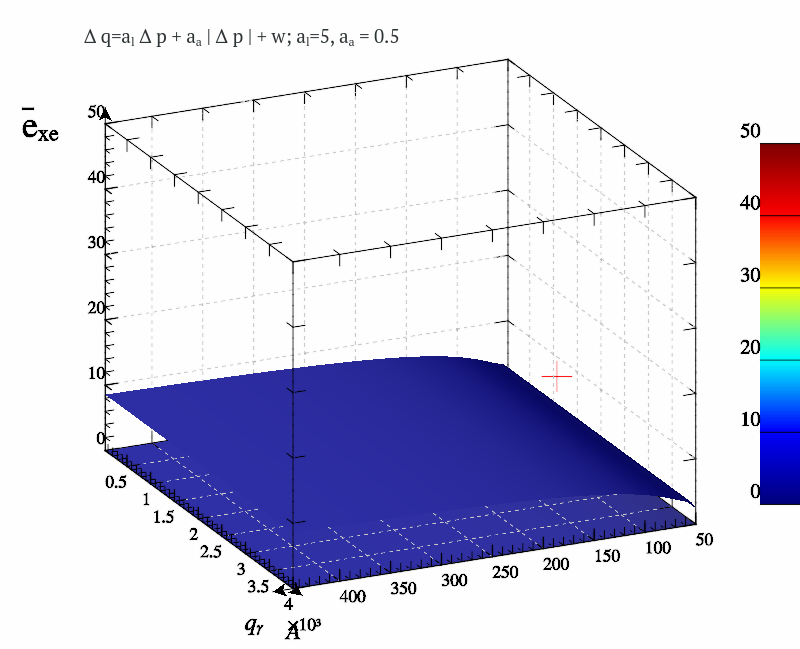
\includegraphics[width=32\TW]{p/lar_e-0-p_exe_A_qg.png}
    \end{center}
    \begin{center}
      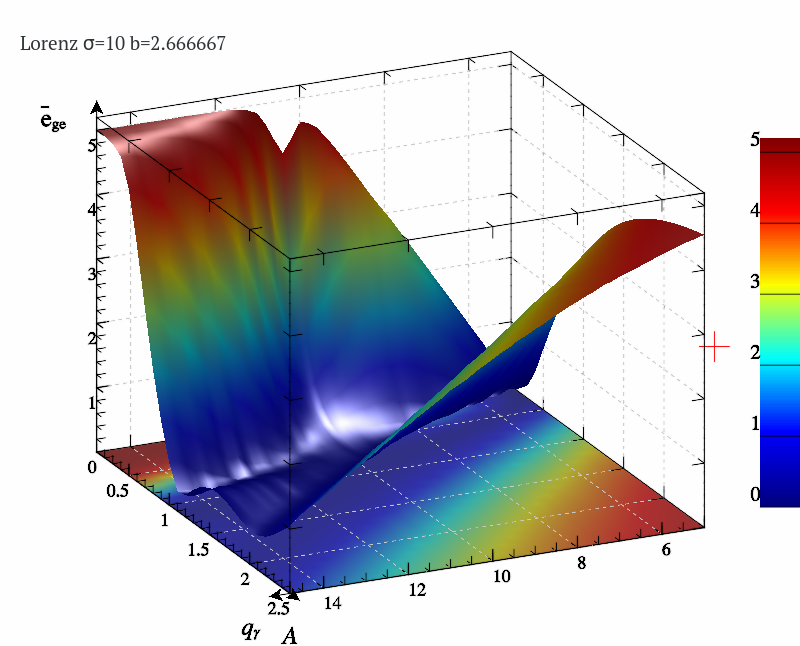
\includegraphics[width=32\TW]{p/lor_e-x1-p_ege_A_qg.png}
      \hfill
      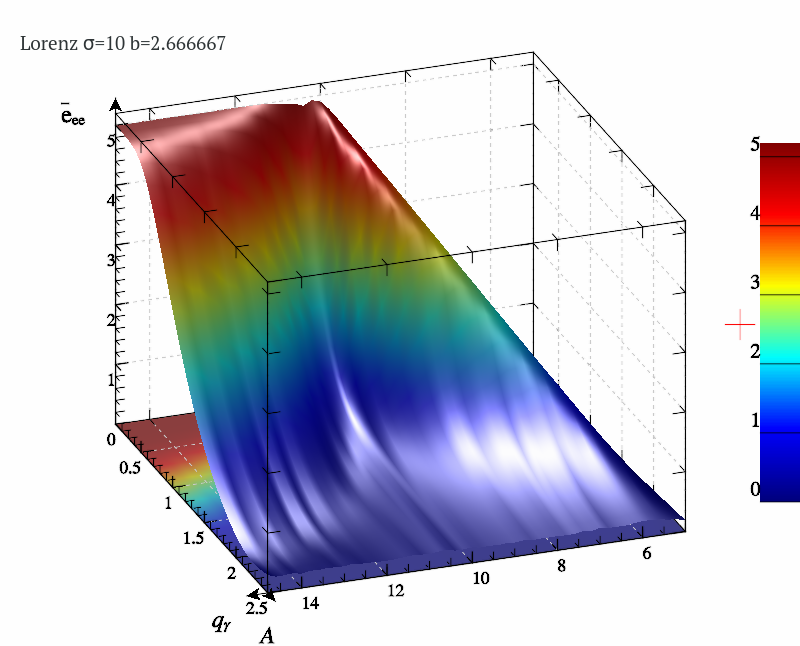
\includegraphics[width=32\TW]{p/lor_e-x1-p_eee_A_qg.png}
      \hfill
      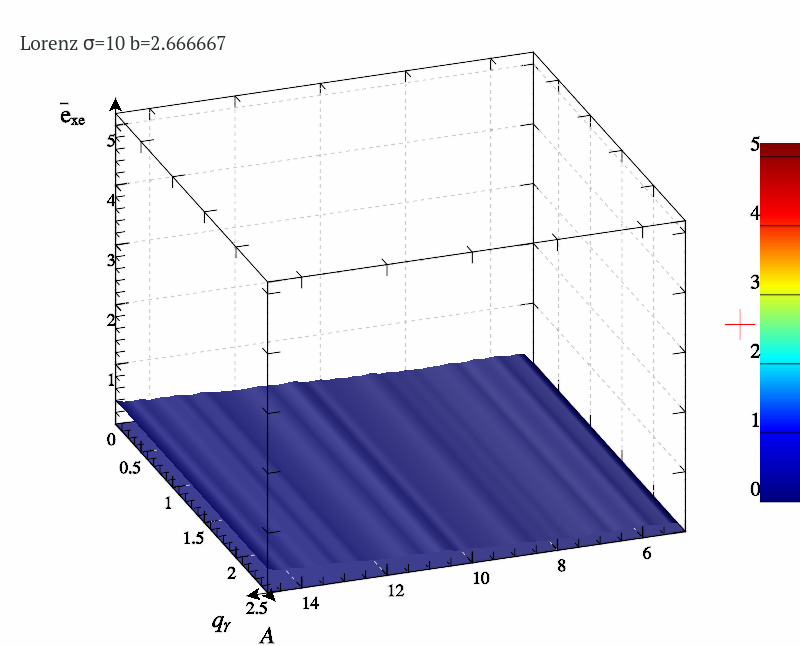
\includegraphics[width=32\TW]{p/lor_e-x1-p_exe_A_qg.png}
    \end{center}
    \caption{Зависимости $\overline{e}_{*}(A,q_\gamma) $ для модели $ \Delta q = a_l \Delta p + a_a |\Delta p| + w $ и системы Лоренца}
    \label{atu:f:iderr_Aqg}
  \end{figure}

\end{frame}



% -----------------------------------------------------------------------

\begin{frame}
  \frametitle{Ошибки идентификации: фиксированная группа (2)}
  %\framesubtitle{}

  \begin{figure}[htb!]
    \begin{center}
      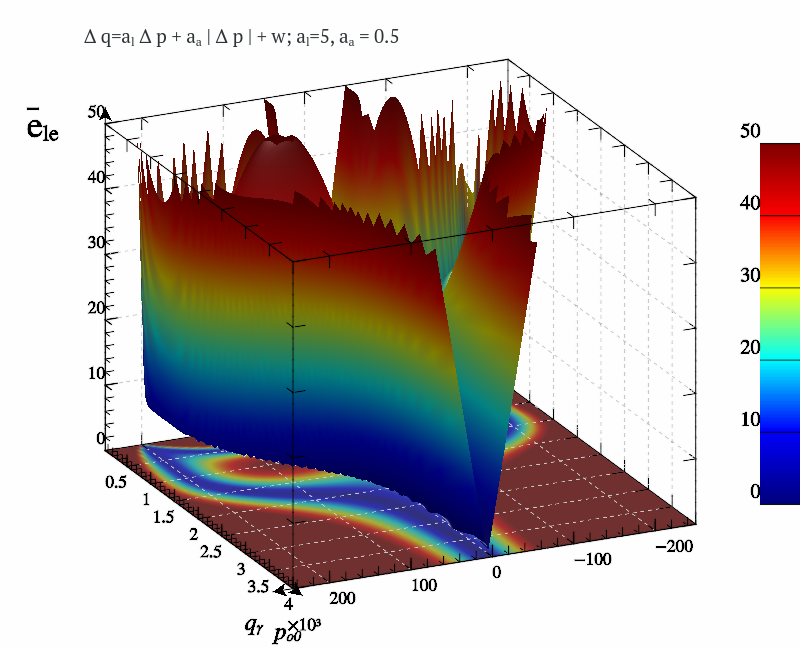
\includegraphics[width=32\TW]{p/lar_e-0-p_ele_po0_qg.png}
      \hfill
      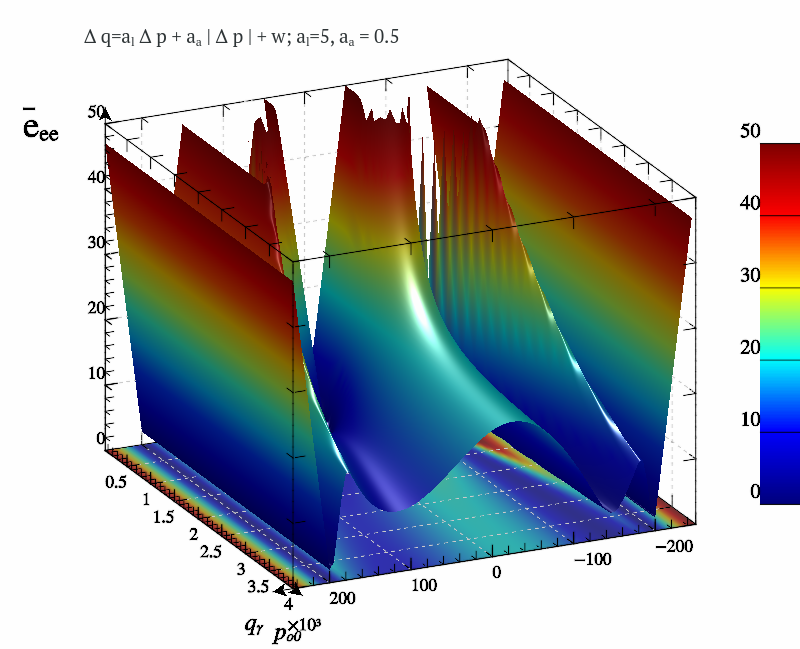
\includegraphics[width=32\TW]{p/lar_e-0-p_eee_po0_qg.png}
      \hfill
      \includegraphics[width=32\TW]{p/lar_e-0-p_exe_po0_qg.png}
    \end{center}
    \begin{center}
      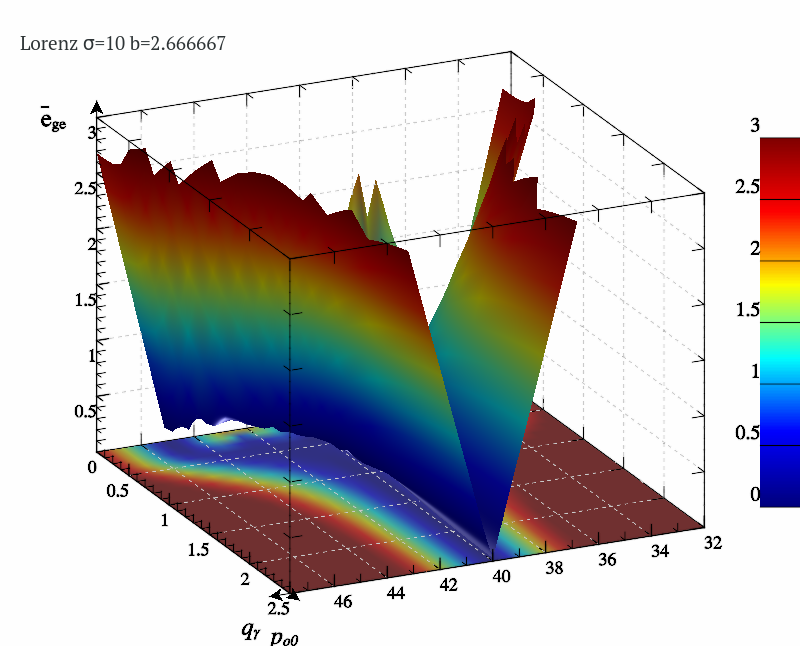
\includegraphics[width=32\TW]{p/lor_e-x1-p_ege_po0_qg.png}
      \hfill
      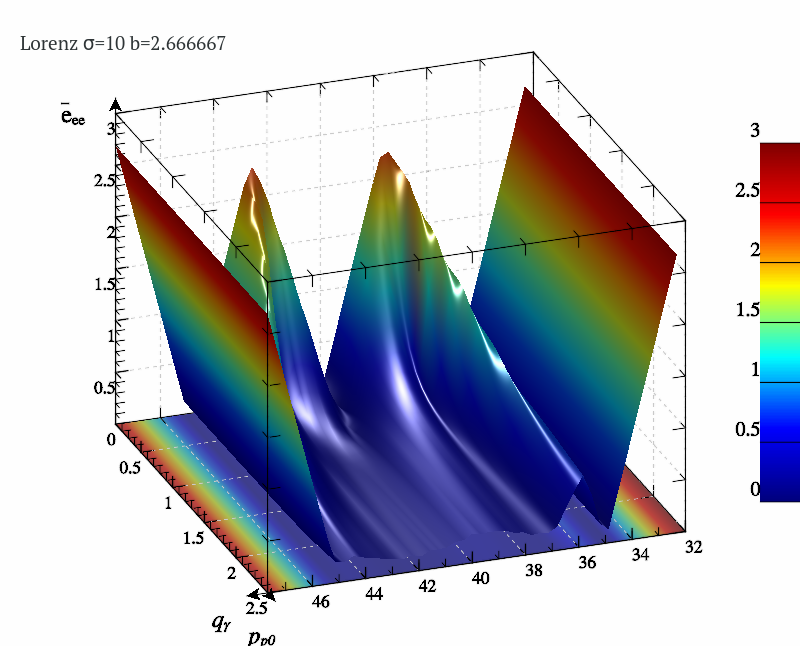
\includegraphics[width=32\TW]{p/lor_e-x1-p_eee_po0_qg.png}
      \hfill
      \includegraphics[width=32\TW]{p/lor_e-x1-p_exe_po0_qg.png}
    \end{center}
    \caption{Зависимости $\overline{e}_{*}(p_{o0},q_\gamma) $ для модели $ \Delta q = a_l \Delta p + a_a |\Delta p| + w $ и системы Лоренца}
    \label{atu:f:iderr_po0qg}
  \end{figure}

\end{frame}





% -----------------------------------------------------------------------
% ------------------------------- P4 ----------------------------------------

\begin{frame}
  \frametitle{Система моделирования ``qontrol''}
  %\framesubtitle{}

  Задачи системы


\end{frame}



% -----------------------------------------------------------------------

\begin{frame}
  \frametitle{Основные особенности программы ``qontrol''}
  %\framesubtitle{}


\end{frame}



% -----------------------------------------------------------------------

\begin{frame}
  \frametitle{Интерфейс программы ``qontrol''}
  %\framesubtitle{}


\end{frame}



% -----------------------------------------------------------------------

\begin{frame}
  \frametitle{Программно-аппаратная реализация взаимодействия с физическими объектами}
  %\framesubtitle{}


\end{frame}



% -----------------------------------------------------------------------

\begin{frame}
  \frametitle{Программно-аппаратная реализация }
  \framesubtitle{Оборудование}


\end{frame}


% -----------------------------------------------------------------------

\begin{frame}
  \frametitle{Программно-аппаратная реализация }
  \framesubtitle{Интерфейс}


\end{frame}



% ----------------------------- P5 ------------------------------------------

% --- lor ---
\begin{frame}
  \frametitle{Система Лоренца}
  \framesubtitle{Определение}

Задача о тепловой конвекции жидкости в плоском слое. Исходная система уравнений:
%
  \begin{equation}
  \begin{cases}
    \pd{\vec{v}}{t} + ( \vec{v} \nabla ) \vec{v} = - \frac{\nabla p}{\rho} + \nu \Delta \vec{v} + \vec{g}, \\
    \pd{\rho}{t} + \nabla ( \rho \vec{v} ) = 0 , \\
    \pd{T}{t} +\nabla ( T \vec{v} ) = \chi \Delta T , \\
    \rho = \rho_0 \left( 1 - \gamma (T - T_0) \right) .
  \end{cases}
  \label{atu:eq:lor_gidro}
  \end{equation}
  %
  где
  $\vec{v} $   -- поле скоростей,
  $T$ -- поле температуры,
  $T_0$ и $T_0+\Delta T$   -- температуры на верхней и нижней границе соответственно,
  $\rho$ и $p$ -- поля плотности и давления,
  $g$ -- ускорение свободного падения,
  $\nu$, $\chi$, $\gamma$  -- коэффициенты кинематической вязкости, температуропроводности и
  теплового расширения соответственно.

%
  \begin{equation}
  \begin{cases}
    \dot{x} = \sigma (y-x ) , \\
    \dot{y} = x (r-z) - y , \\
    \dot{z} = x y - b z .
  \end{cases}
  \label{atu:eq:lor}
  \end{equation}

\end{frame}



% -----------------------------------------------------------------------

\begin{frame}
  \frametitle{Система Лоренца}
  \frametitle{Свойства}

  Демонстрирует затухающую, хаотическую и сложно-периодическую динамику.

  \begin{figure}[h!]
  \begin{center}
    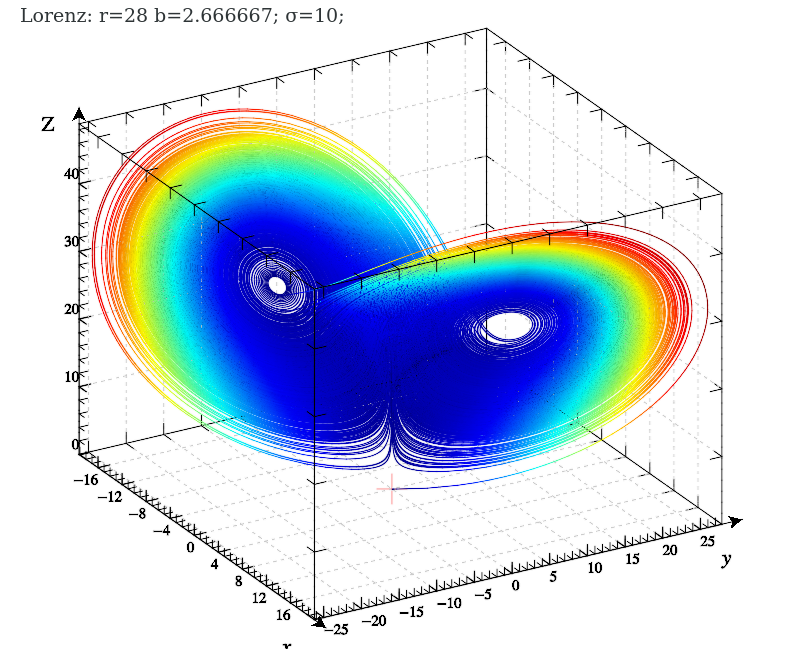
\includegraphics[width=0.49\textwidth]{p/lor/lor0-p_xyz_r=028.png}
    \hfill
    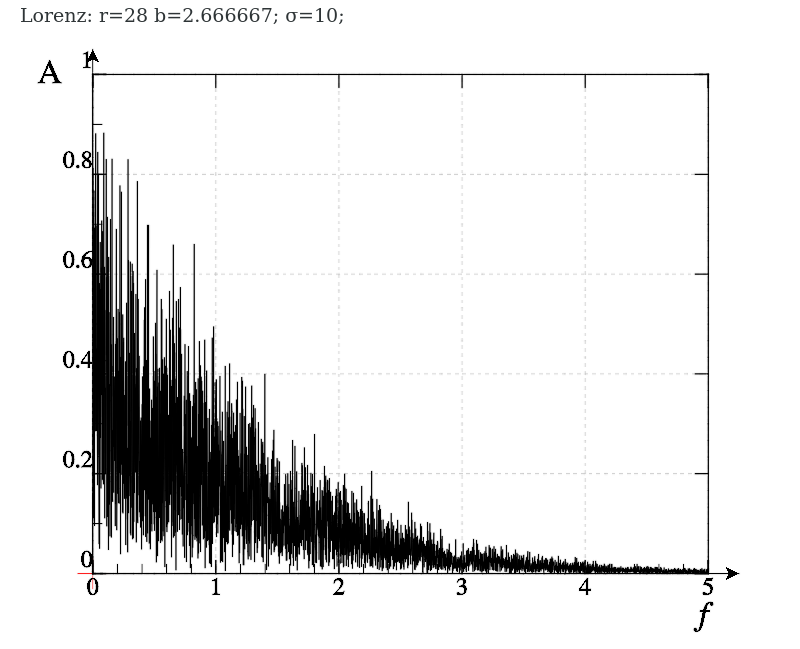
\includegraphics[width=0.49\textwidth]{p/lor/lor0_fft-p_f_r=028.png}
  \end{center}
    \caption{Аттрактор и спектр системы Лоренца (\ref{atu:eq:lor}) в хаотическом режиме ($r=28$)}
  \label{atu:f:lor_attractor_phase_chaos28}
  \end{figure}

\end{frame}



% -----------------------------------------------------------------------

\begin{frame}
  \frametitle{Система Лоренца}
  \framesubtitle{Анализ критериев}


  \begin{figure}[h!]
    \centerline{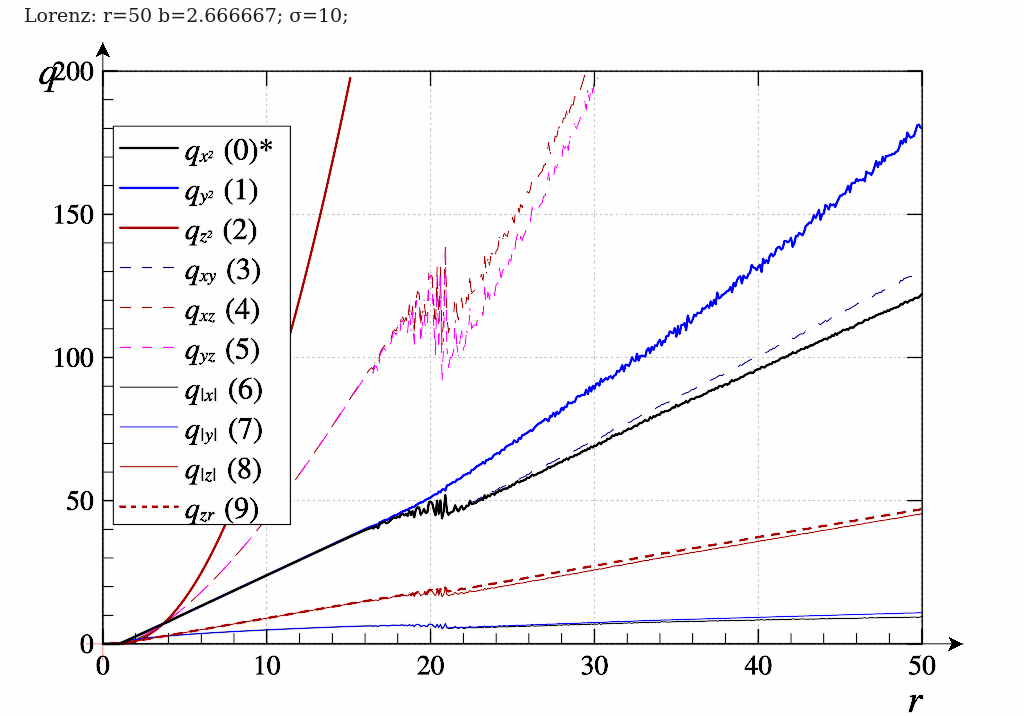
\includegraphics[width=54\TW]{p/lor/lor_q-p_q_r.png} }
    \caption{Рассматриваемые критерии для системы Лоренца}
    \label{atu:f:lor_q}
  \end{figure}

В дальнейших исследованиях ограничимся
критериями
  $q_{x^2}$, ${q_{x}}$ и $q_{y^2}$.

\end{frame}



% -----------------------------------------------------------------------

\begin{frame}
  \frametitle{Система Лоренца}
  \framesubtitle{Зависимости $\sigma_{q}(\ldots)$ и тестовая задача}
  \begin{figure}[h!]
  \begin{center}
    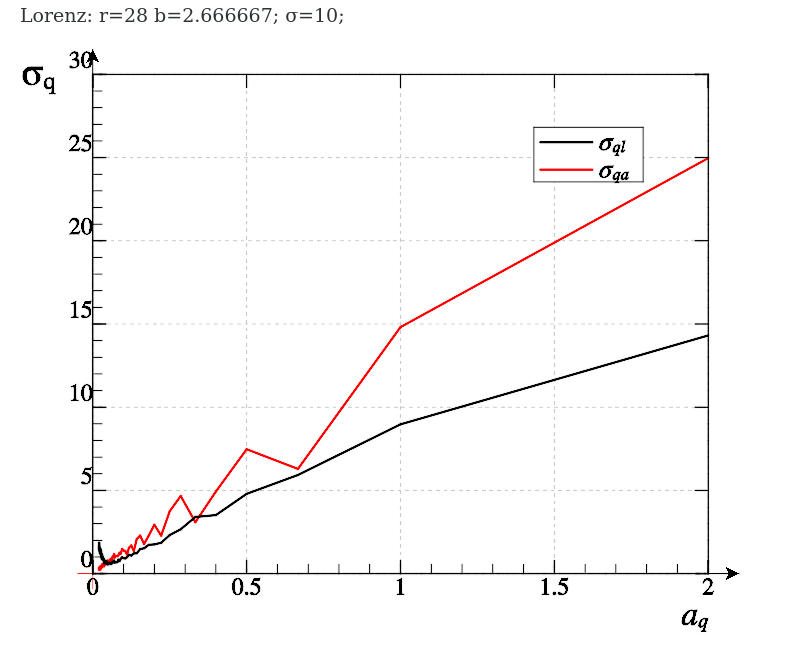
\includegraphics[width=0.49\textwidth]{p/lor/lor_qx2_tau-p_aq_sd.png}
    \hfill
    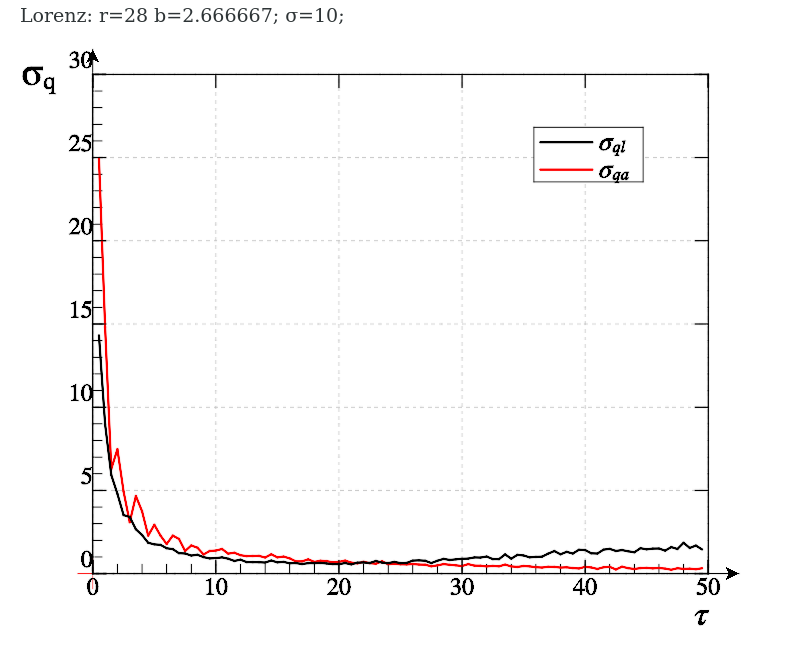
\includegraphics[width=0.49\textwidth]{p/lor/lor_qx2_tau-p_tau_sd.png}
  \end{center}
  \caption{Зависимости $\sigma_{q}(a_q)$ и $\sigma_{q}(\tau_q)$ для системы Лоренца, критерий $q_{x^2}$}
  \label{atu:f:lor_qx2_tau}
  \end{figure}

  \vspace{-3ex}
  \[
    p(t) \in [20, 60],
  \]
  %
  \begin{equation}
    r_o(t) = p_o(t) = p_0 +  U_{p} \sign \sin( \omega_{p} t ),
    \label{atu:eq:lor_po_t_sign}
  \end{equation}
  %
  %
  \begin{equation}
    r_o(t) = p_o(t) = p_0 +  U_{p} \sin( \omega_{p} t ),
    \label{atu:eq:lor_po_t_sin}
  \end{equation}
  %
  где:
  $p_0 = 37$, $U_p=12$, $\omega_p=0.09$.

\end{frame}



% -----------------------------------------------------------------------

\begin{frame}
  \frametitle{Система Лоренца}
  \framesubtitle{Идентификация методом  Fblvd1.2.$q_{x2}$ }


\begin{figure}[h!]
  \centerline{
    \includegraphics[width=0.49\textwidth]{p/lor/Fblvd1_2-p_xz_1_wp009.png}
    \hfill
    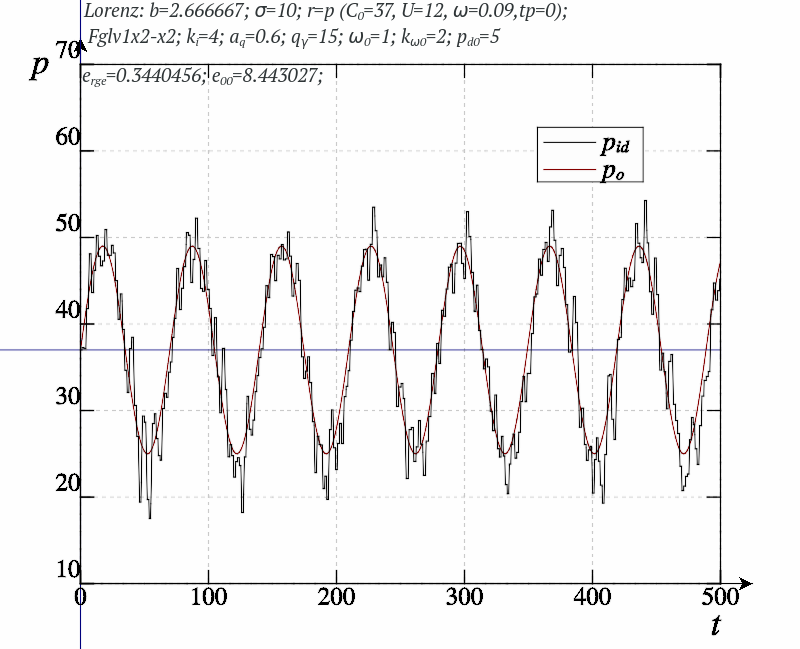
\includegraphics[width=0.49\textwidth]{p/lor/Fblvd1_2-p_xz_0_wp009.png}
  }
  \caption{Процесс идентификации параметра ``$r$'' системы Лоренца методом Fblvd1.2.$q_{x^2}$ при условиях~(\ref{atu:eq:lor_po_t_sign}) и (\ref{atu:eq:lor_po_t_sin})}
  \label{atu:f:lor_id_Fblvd1}
\end{figure}

\end{frame}



% -----------------------------------------------------------------------

\begin{frame}
  \frametitle{Система Лоренца}
  \framesubtitle{Идентификация методом qAuv5.3r.$q_{x2}$}


  \begin{figure}[h!]
    \centerline{
      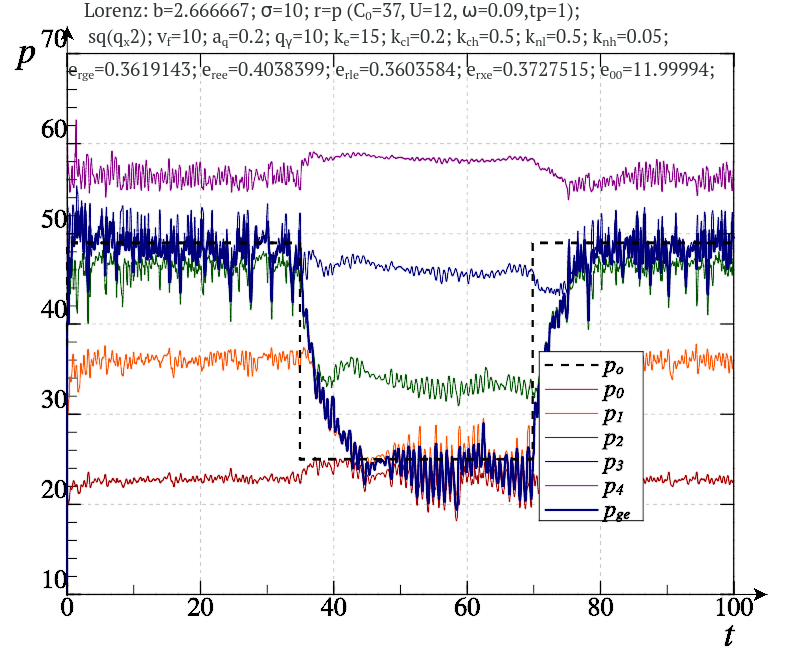
\includegraphics[width=0.49\textwidth]{p/lor/lor_qAuv5_3r_qx2-p_t_pi_sign.png}
      \hfill
      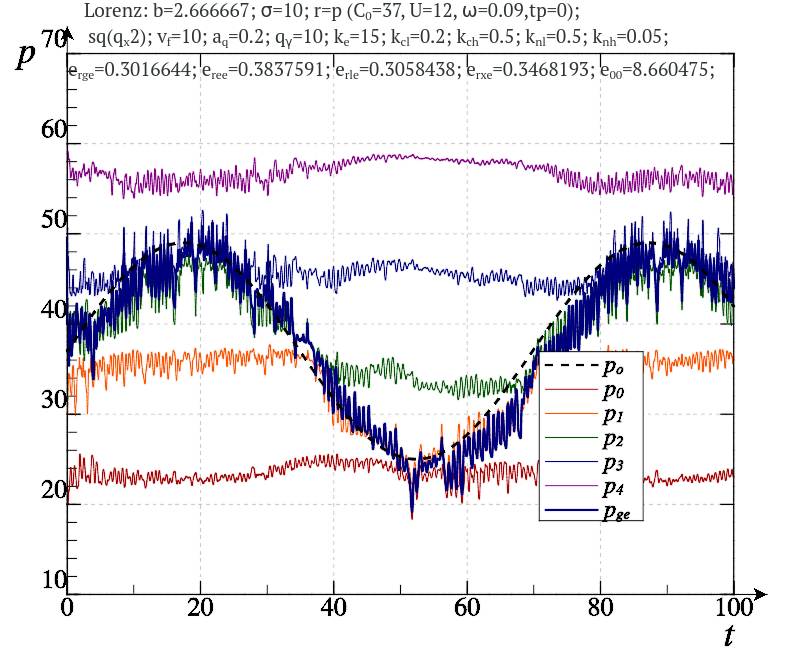
\includegraphics[width=0.49\textwidth]{p/lor/lor_qAuv5_3r_qx2-p_t_pi_sin.png}
    }
    \caption{Процесс идентификации параметра ``$r$'' системы Лоренца методом qAuv5.3r.$q_{x^2}$ при условии~(\ref{atu:eq:lor_po_t_sign})}
    \label{atu:f:lor_id_qAuv5.3r.q_x2_sign}
  \end{figure}

\end{frame}



% -----------------------------------------------------------------------

\begin{frame}
  \frametitle{Система Лоренца}
  \framesubtitle{Идентификация методом FAlv5.3z.$q_{x2}$}


  \begin{figure}[h!]
    \centerline{
      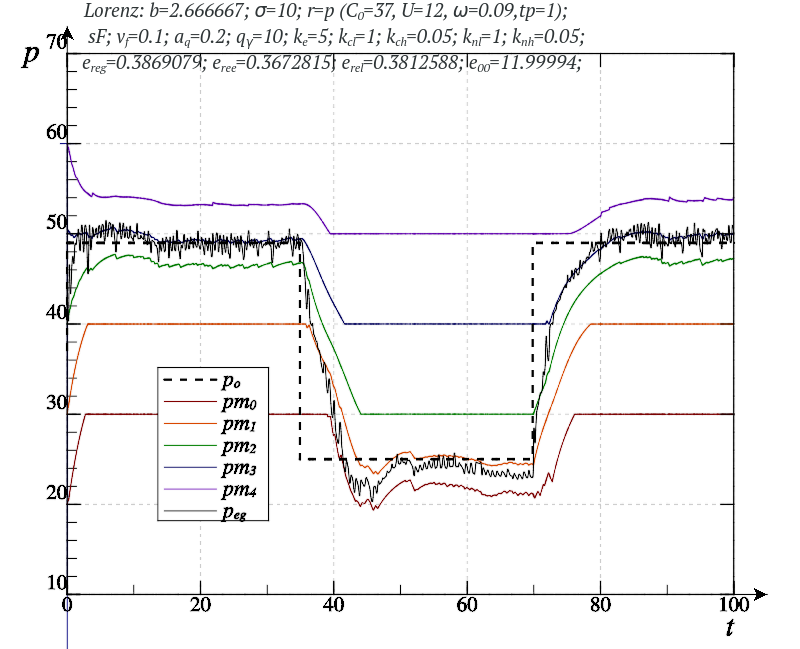
\includegraphics[width=0.49\textwidth]{p/lor/lor_FAlv5_3z_qx2-pl_n_sign.png}
      \hfill
      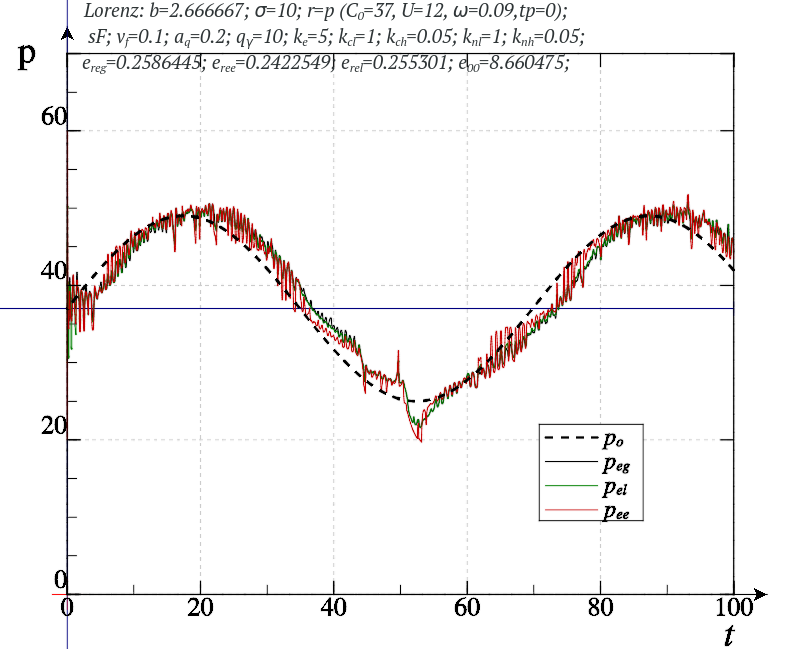
\includegraphics[width=0.49\textwidth]{p/lor/lor_FAlv5_3z_qx2-p_p_sin.png}
    }
    \caption{Процесс идентификации параметра ``$r$'' системы Лоренца методом FAlv5.3z.$q_{x^2}$ при условии~(\ref{atu:eq:lor_po_t_sign})}
    \label{atu:f:lor_id_FAlv5.3z.q_x2_sign}
  \end{figure}


\end{frame}



% -----------------------------------------------------------------------

\begin{frame}
  \frametitle{Система Лоренца}
  \framesubtitle{Зависимости $\overline{e}(a_q)$}

  \begin{figure}[h!]
    \centerline{
      {~}\hfill
      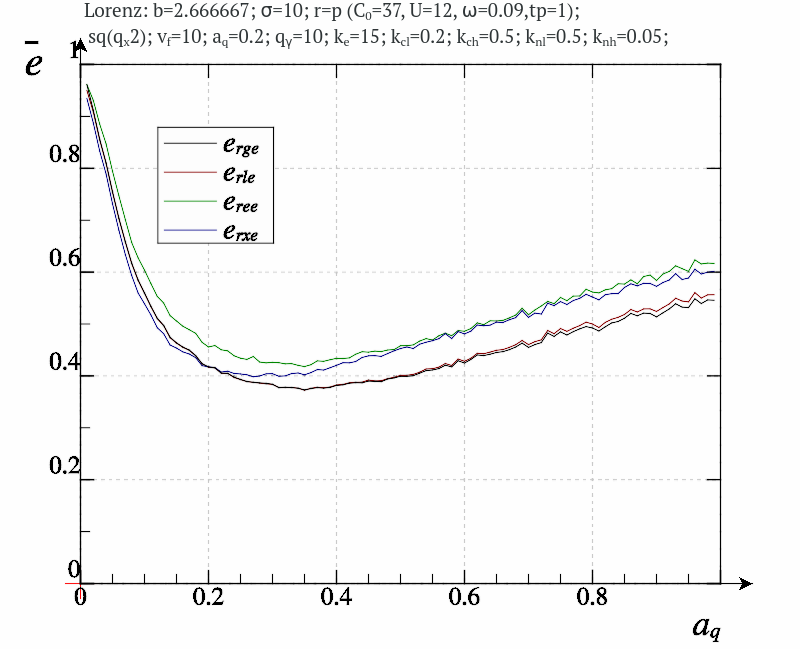
\includegraphics[width=\DDW]{p/lor/lor_qAuv5_3r_qx2-p_a_q_e_sign.png}
      \hfill
      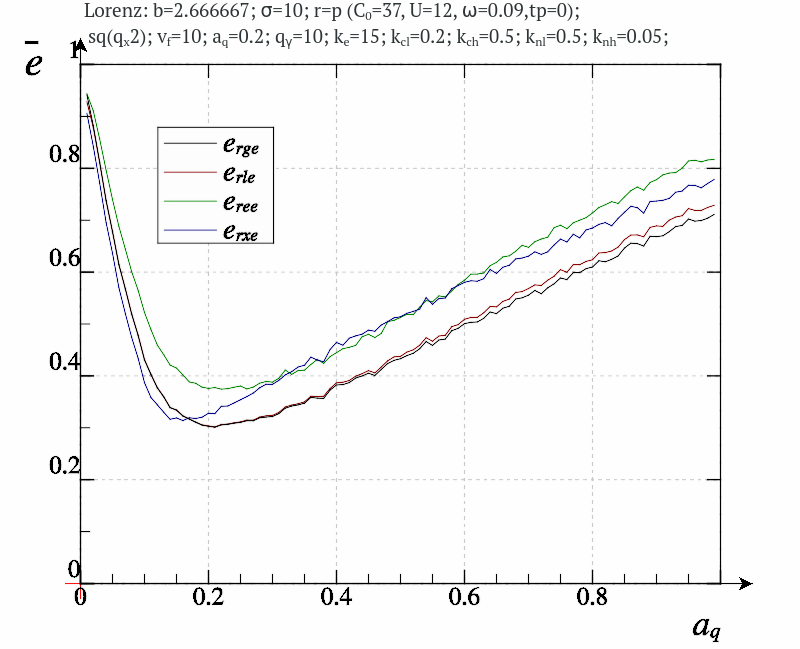
\includegraphics[width=\DDW]{p/lor/lor_qAuv5_3r_qx2-p_a_q_e_sin.png}
      \hfill{~}
    }
    \centerline{
      {~}\hfill
      \includegraphics[width=\DDW]{p/lor/lor_FAlv5_3z_qx2-p_a_q_e_sign.png}
      \hfill
      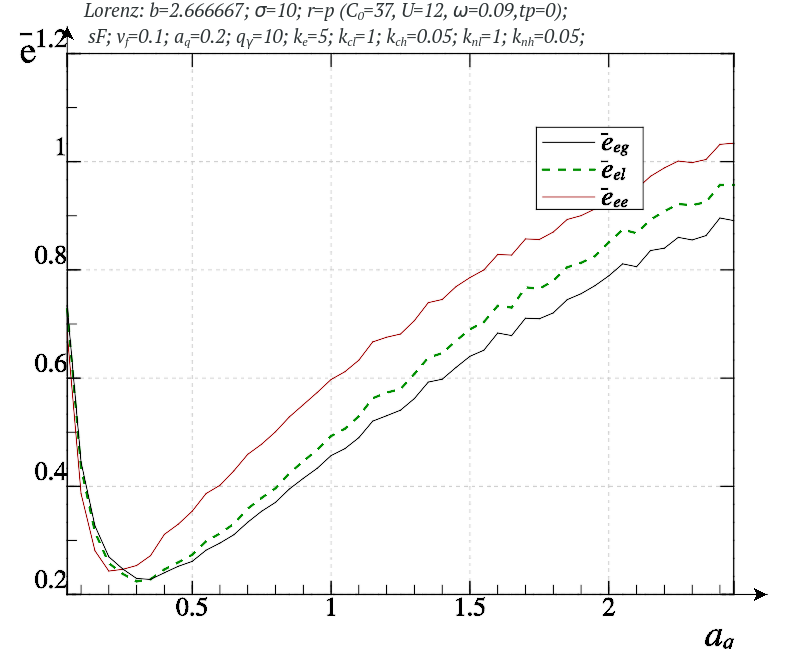
\includegraphics[width=\DDW]{p/lor/lor_FAlv5_3z_qx2-p_a_q_e_sin.png}
      \hfill{~}
    }
    \caption{Зависимости $\overline{e}_{r*}(a_q)$ при идентификации системы Лоренца методами qAuv5.3r.$q_{x^2}$ и FAlv5.3z.$q_{x^2}$
     при~(\ref{atu:eq:lor_po_t_sign}) и (\ref{atu:eq:lor_po_t_sin})}
    \label{atu:f:lor_a_q_Fq.q_x2}
  \end{figure}


\end{frame}



% -----------------------------------------------------------------------

\begin{frame}
  \frametitle{Система Лоренца}
  \framesubtitle{Зависимости $\overline{e}(q_\gamma)$}

  \begin{figure}[h!]
    \centerline{
      {~}\hfill
      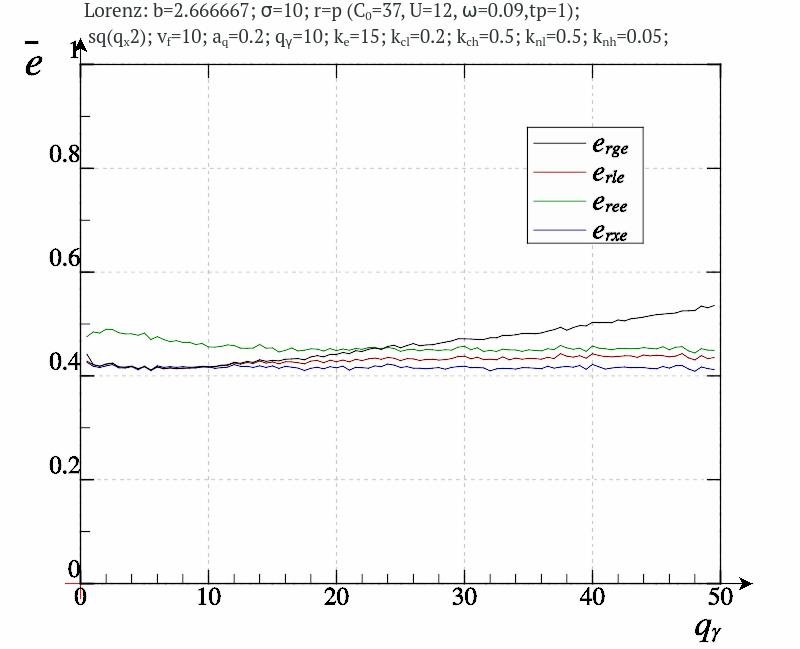
\includegraphics[width=\DDW]{p/lor/lor_qAuv5_3r_qx2-p_qgamma_e_sign.png}
      \hfill
      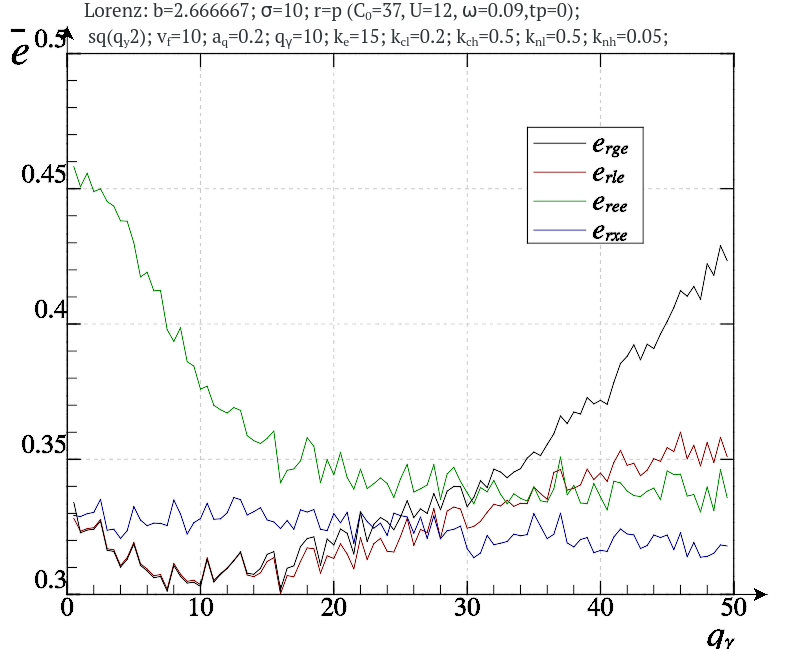
\includegraphics[width=\DDW]{p/lor/lor_qAuv5_3r_qx2-p_qgamma_e_sin.png}
      \hfill{~}
    }
    \centerline{
      {~}\hfill
      \includegraphics[width=\DDW]{p/lor/lor_FAlv5_3z_qx2-p_qg_e_sign.png}
      \hfill
      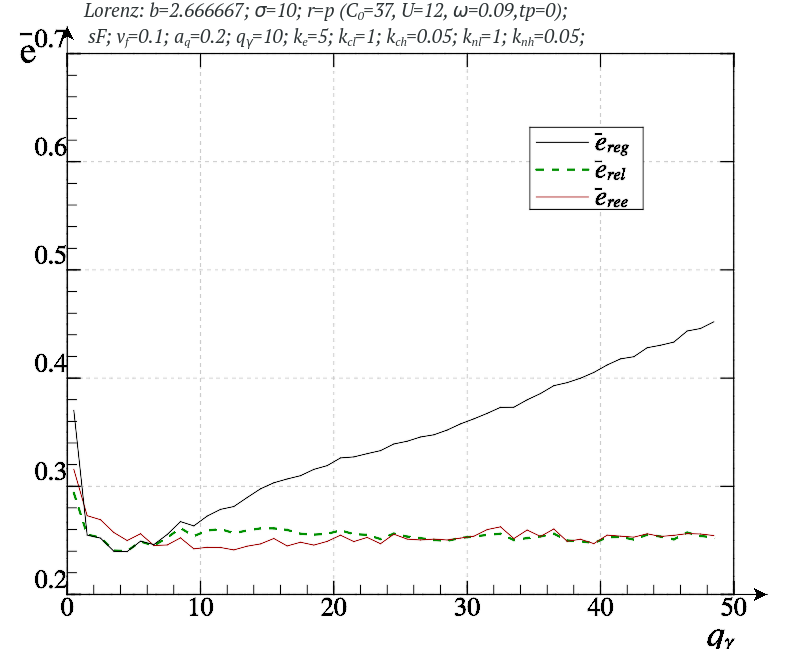
\includegraphics[width=\DDW]{p/lor/lor_FAlv5_3z_qx2-p_qg_e_sin.png}
      \hfill{~}
    }
    \caption{Зависимости $\overline{e}_{r*}(q_\gamma)$
     при идентификации системы Лоренца методами qAuv5.3r.$q_{x^2}$ и FAlv5.3z.$q_{x^2}$
     при~(\ref{atu:eq:lor_po_t_sign}) и (\ref{atu:eq:lor_po_t_sin})}
    \label{atu:f:lor_qgamma_Fq.q_x2}
  \end{figure}



\end{frame}

% -----------------------------------------------------------------------

\begin{frame}
  \frametitle{Система Лоренца}
  \framesubtitle{Зависимости $\overline{e}(v_f)$}


  \begin{figure}[h!]
    \centerline{
      {~}\hfill
      \includegraphics[width=\DDW]{p/lor/lor_qAuv5_3r_qx2-p_v_f_e_sign.png}
      \hfill
      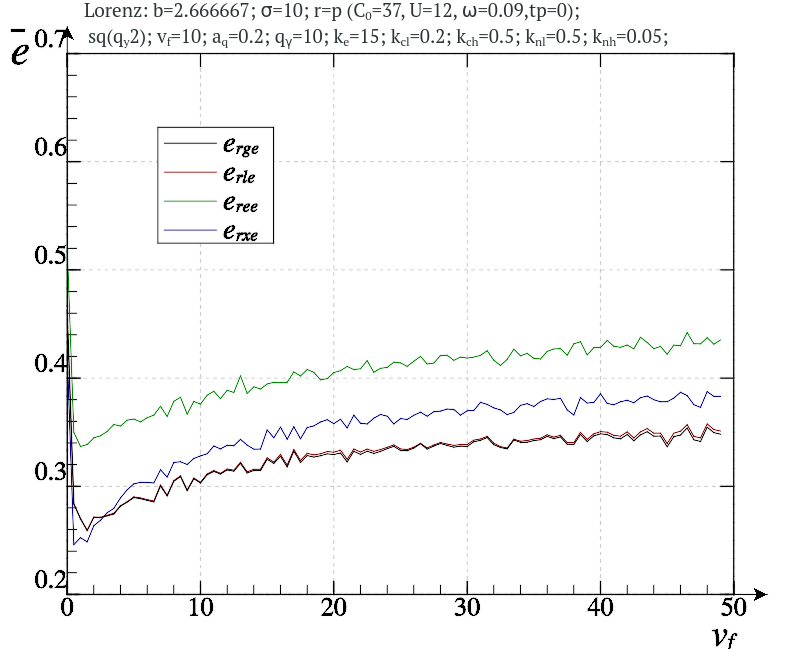
\includegraphics[width=\DDW]{p/lor/lor_qAuv5_3r_qx2-p_v_f_e_sin.png}
      \hfill{~}
    }
    \centerline{
      {~}\hfill
      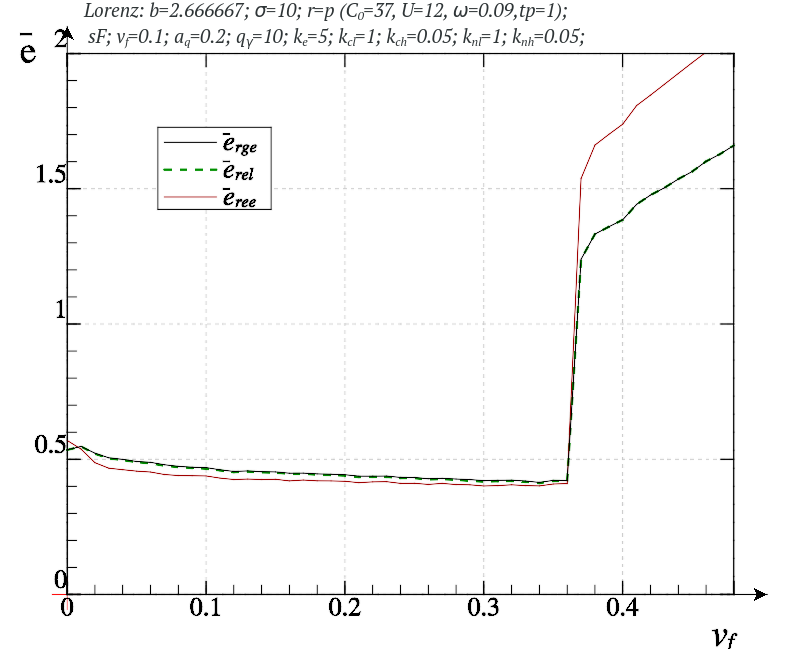
\includegraphics[width=\DDW]{p/lor/lor_FAlv5_3z_qx2-p_v_f_e_sign.png}
      \hfill
      \includegraphics[width=\DDW]{p/lor/lor_FAlv5_3z_qx2-p_v_f_e_sin.png}
      \hfill{~}
    }
    \caption{Зависимости $\overline{e}_{r*}(v_f)$
     при идентификации системы Лоренца методами qAuv5.3r.$q_{x^2}$ и FAlv5.3z.$q_{x^2}$
     при~(\ref{atu:eq:lor_po_t_sign}) и (\ref{atu:eq:lor_po_t_sin})}
    \label{atu:f:lor_vf_Fq.q_x2}
  \end{figure}


\end{frame}


% -----------------------------------------------------------------------

\begin{frame}
  \frametitle{Система Лоренца}
  \framesubtitle{Влияние вида функции качества на процесс идентификации}

  \begin{figure}[h!]
    \centerline{
      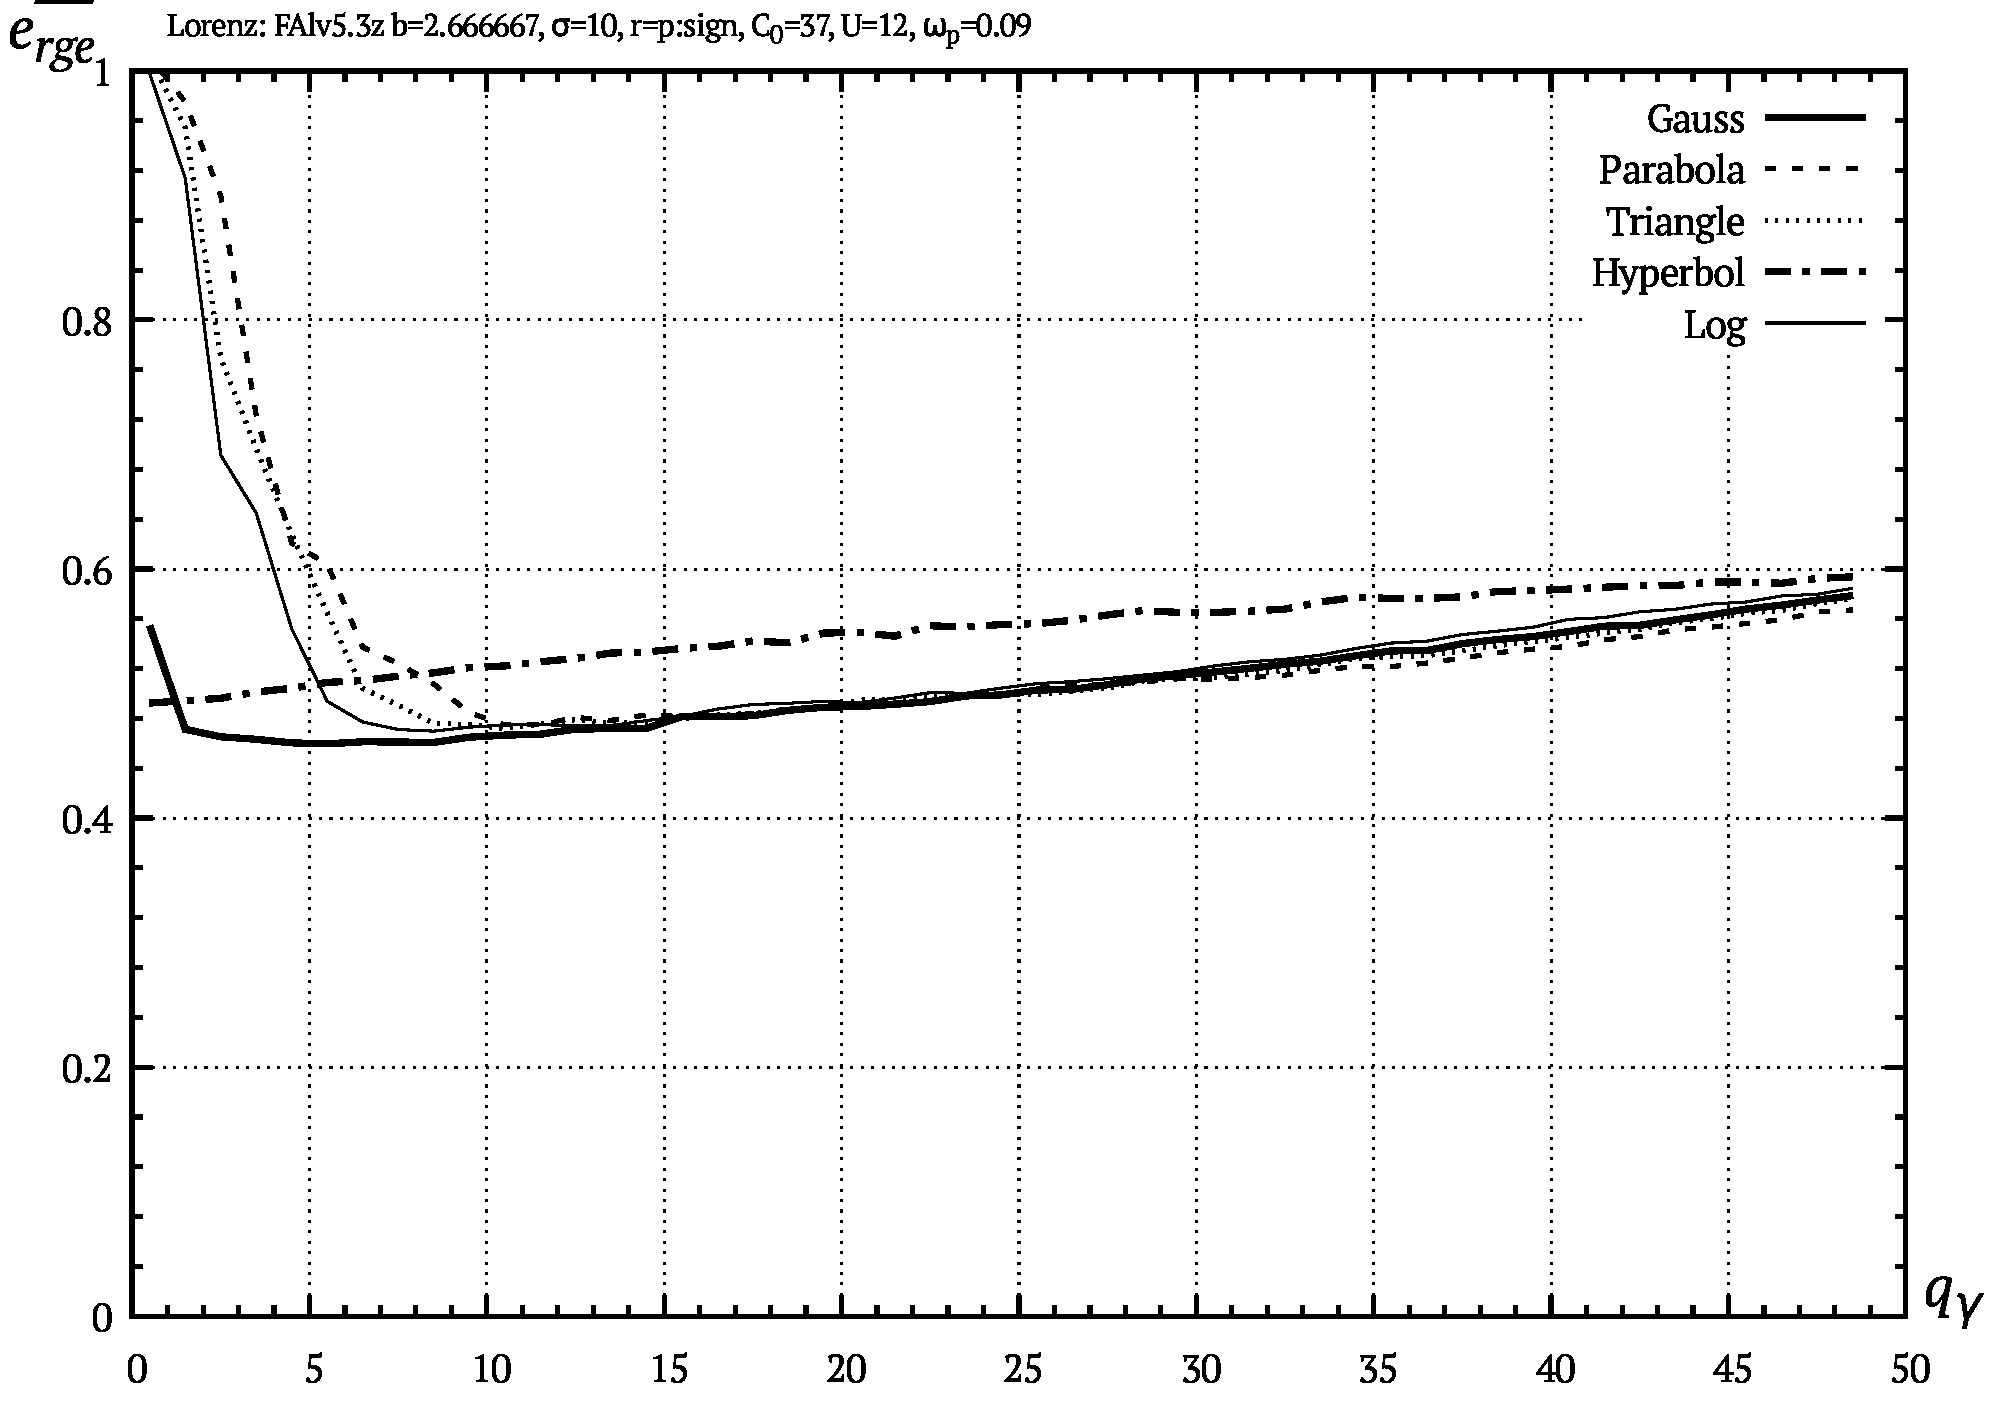
\includegraphics[width=0.49\textwidth]{p/lor/lor_FAlv5_3z_qx2_Ft-p_qg_e_all_sign_rge.png}
      \hfill
      \includegraphics[width=0.49\textwidth]{p/lor/lor_FAlv5_3z_qx2_Ft-p_qg_e_all_sin_rge.png}
    }
    \caption{Семейства зависимостей $\overline{e}_{rge}(q_\gamma)$ для различных видов функций качества при идентификации системы Лоренца методом FAlv5.3z.$q_{x^2}$
     при~(\ref{atu:eq:lor_po_t_sign}) и (\ref{atu:eq:lor_po_t_sin})}
    \label{atu:f:lor_ftype_rge}
  \end{figure}

\end{frame}


% -----------------------------------------------------------------------

\begin{frame}
  \frametitle{Система Лоренца}
  \framesubtitle{Влияние количества поисковых агентов на процесс идентификации}


  \begin{figure}[h!]
    \centerline{
      \includegraphics[width=0.49\textwidth]{p/lor/lor_FAlvN_3z_qx2_p_qg_e_rge_sign.png}
      \hfill
      \includegraphics[width=0.49\textwidth]{p/lor/lor_FAlvN_3z_qx2_p_qg_e_rge_sin.png}
    }
    \caption{Семейства зависимостей $\overline{e}_{rge}(q_\gamma)$ для различных значений $N$ при идентификации системы Лоренца методом FAlv5.3r.$q_{x^2}$
     при~(\ref{atu:eq:lor_po_t_sign}) и (\ref{atu:eq:lor_po_t_sin})}
    \label{atu:f:lor_N_rge}
  \end{figure}


\end{frame}


% -----------------------------------------------------------------------

\begin{frame}
  \frametitle{Система Лоренца}
  \framesubtitle{Зависимости критерив от двух параметров}


  \begin{figure}[h!]
    \centerline{
      {~}\hfill
      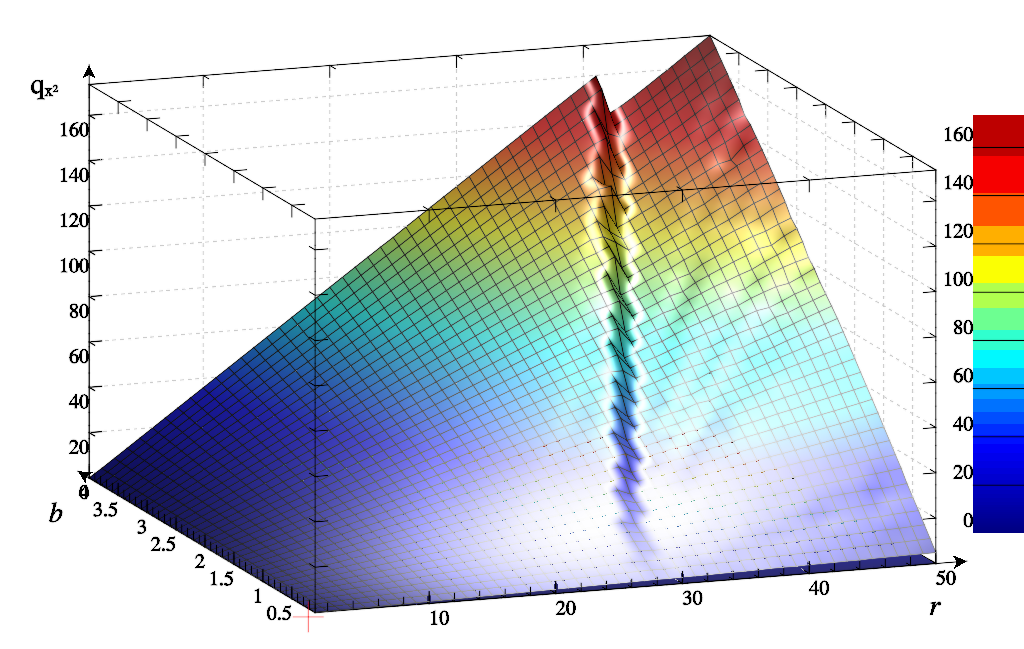
\includegraphics[width=\DDW]{p/lor/lor_qx2_r_b.png}
      \hfill
      \includegraphics[width=\DDW]{p/lor/lor_qy2_r_b.png}
      \hfill{~}
    }
    \centerline{
      {~}\hfill
      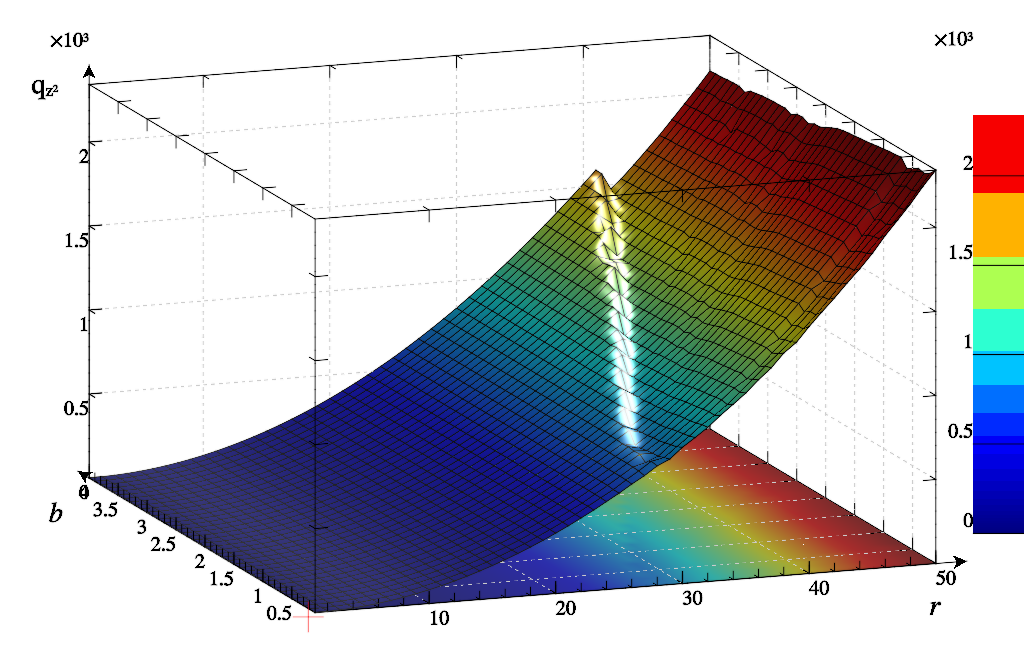
\includegraphics[width=\DDW]{p/lor/lor_qz2_r_b.png}
      \hfill
      \includegraphics[width=\DDW]{p/lor/lor_qxmy2_r_b.png}
      \hfill{~}
    }
    \caption{Зависимости $q_{*}(r,b)$ для системы Лоренца }
    \label{atu:f:lor_qrb}
  \end{figure}


\end{frame}



% -----------------------------------------------------------------------

% ---- spr_a ----
\begin{frame}
  \frametitle{Система Sprott A}
  \framesubtitle{Определение}

  Задаётся системой уравнений:
  %
  \begin{equation}
    \begin{cases}
      \dot{x} =  y, \\
      \dot{y} = -x + yz, \\
      \dot{z} =  1 - y^2.
    \end{cases}
    \label{atu:eq:spr_a_orig}
  \end{equation}

  Отличительной особенностью
  этой системы является отсутствие положений равновесия, что делает
  невозможным применение многих известных методов анализа, основанных на
  каком-либо разложении в окрестностях точек равновесия.

  Вводим параметр $c_{x_y}$, не изменяя структуры уравнения:
  %
  \begin{equation}
    \begin{cases}
      \dot{x} =  c_{x_y} y, \\
      \dot{y} = -x + yz, \\
      \dot{z} =  1 - y^2.
    \end{cases}
    \label{atu:eq:spr_a}
  \end{equation}
  \end{frame}

% -----------------------------------------------------------------------

\begin{frame}
  \frametitle{Система Sprott A}
  \framesubtitle{Свойства}

  В диапазоне $c_{x_y} \in [0.1 ; 0.7] $
  наблюдаются перестройки структуры аттрактора, а при относительно больших
  значениях данного параметра аттрактор представляет собой полый тор.

  \begin{figure}[htb!]
  \centerline{
    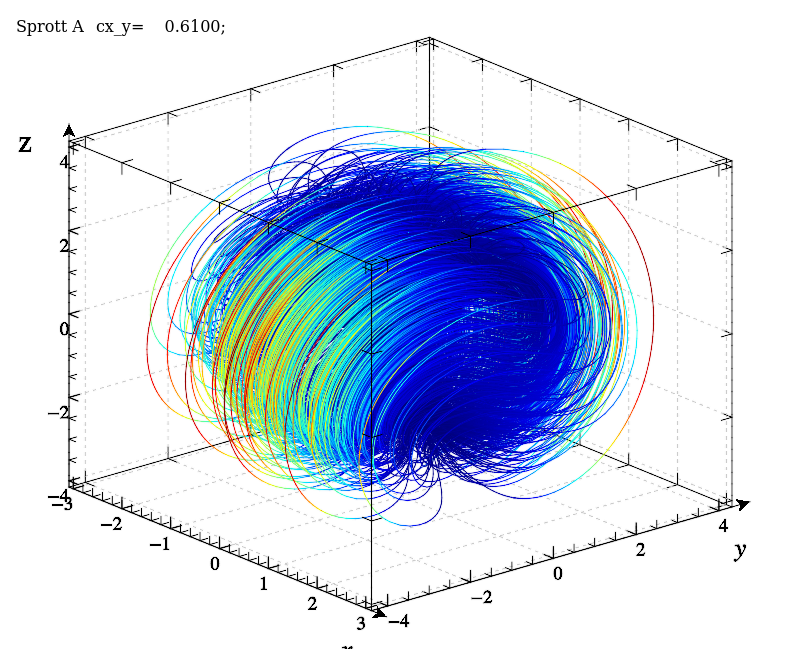
\includegraphics[width=0.49\textwidth]{p/spr_a/sprott_a-p_xyz_cx_y=0x610.png}
    \includegraphics[width=0.49\textwidth]{p/spr_a/sprott_a_f-p_f_cx_y=0x610.png}
  }
  \caption{Аттрактор и спектр системы (\ref{atu:eq:spr_a}) при $ c_{x_y} =0.610 $.
    Хаотический режим
  }
  \label{atu:f:spr_a_p_0610}
  \end{figure}

\end{frame}


% -----------------------------------------------------------------------

\begin{frame}
  \frametitle{Система Sprott A}
  \framesubtitle{Критерии}


  \begin{figure}[htb!]
  \centerline{
    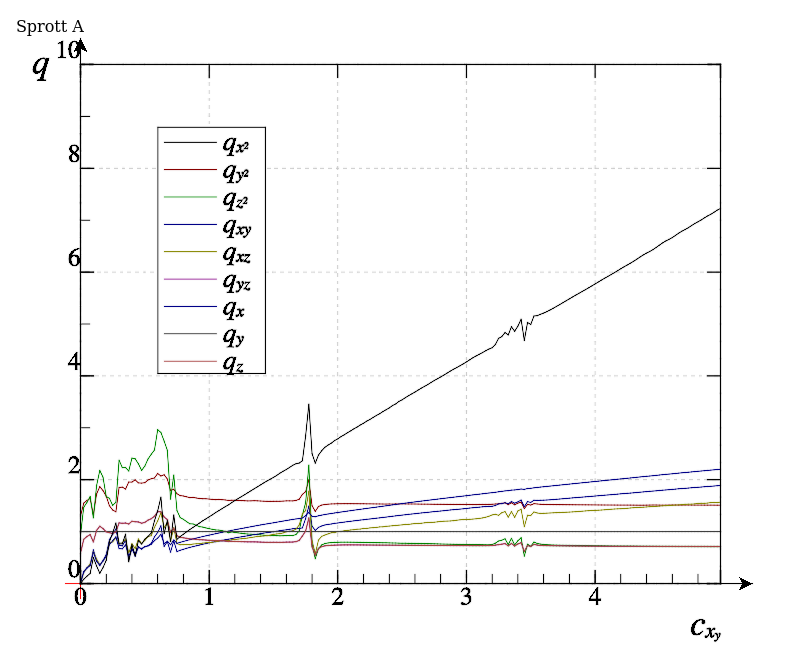
\includegraphics[width=0.50\textwidth]{p/spr_a/sprott_a_q-p_c_x_y.png}
  }
  \caption{Зависимости $q_{*}(c_{x_y})$ для системы (\ref{atu:eq:spr_a}) }
  \label{atu:f:spr_a_q}
  \end{figure}

  \vspace{-4ex}
  Однозначный ответ о возможном виде критерия -- $q_{x^2}$.

  В начальной области
  $q_{x^2}(c_{x_y}) $, а именно там, где происходят постоянные
  перестройки структуры аттрактора, ни один из рассматриваемых критериев
  не имеет достаточной монотонности.
\end{frame}



% -----------------------------------------------------------------------

\begin{frame}
  \frametitle{Система Sprott A}
  \framesubtitle{Идентификация методом qAuv5.3r.$q_{x2}$}


\begin{figure}[h!]
  \centerline{
    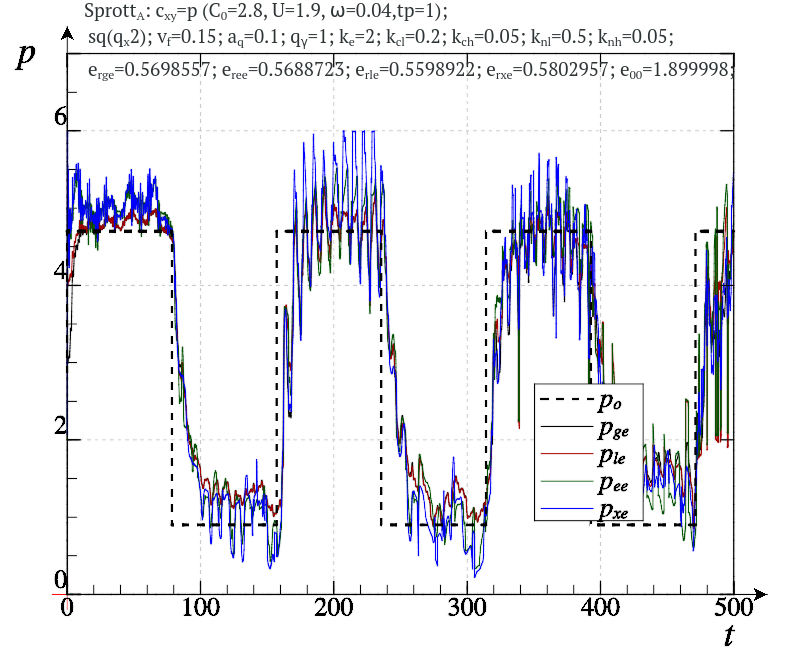
\includegraphics[width=0.49\textwidth]{p/spr_a/sprott_a_qAuv5_3r_qx2-p_t_pz_sign.png}
    \hfill
    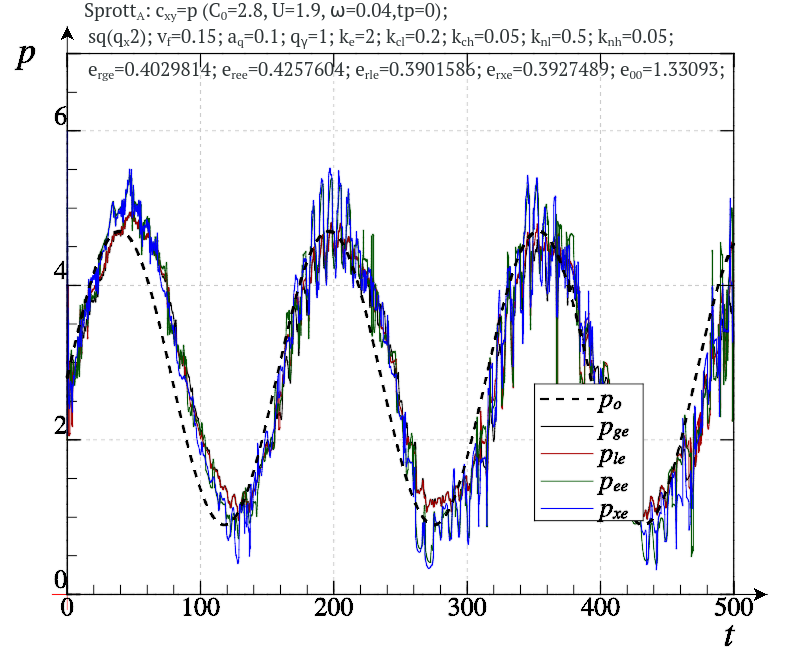
\includegraphics[width=0.49\textwidth]{p/spr_a/sprott_a_qAuv5_3r_qx2-p_t_pz_sin.png}
  }
  \caption{Процесс идентификации параметра ``$c_{x_y}$'' системы Sprott A методом qAuv5.3r.$q_{x^2}$}
  \label{atu:f:spr_a_id_qAuv5.3r.q_x2_sign}
\end{figure}

\end{frame}


% -----------------------------------------------------------------------

\begin{frame}
  \frametitle{Система Sprott A}
  \framesubtitle{Идентификация методом FAlv5.3r.$q_{x2}$}


\begin{figure}[h!]
  \centerline{
    \includegraphics[width=0.49\textwidth]{p/spr_a/sprott_a_FAlv5x3r-p_p_sign.png}
    \hfill
    \includegraphics[width=0.49\textwidth]{p/spr_a/sprott_a_FAlv5x3r-p_p_sin.png}
  }
  \caption{Процесс идентификации параметра ``$c_{x_y}$'' системы Sprott A методом FAlv5.3r.$q_{x^2}$}
  \label{atu:f:spr_a_id_FAlv5.3r.q_x2_sign}
\end{figure}

\end{frame}



% -----------------------------------------------------------------------

\begin{frame}
  \frametitle{Система Sprott A}
  \framesubtitle{Зависимости $\overline{e}(a_q)$}

  \begin{figure}[h!]
    \centerline{
      {~}\hfill
      \includegraphics[width=\DDW]{p/spr_a/sprott_a_qAuv5_3r_qx2-p_a_q_e_sign.png}
      \hfill
      \includegraphics[width=\DDW]{p/spr_a/sprott_a_qAuv5_3r_qx2-p_a_q_e_sin.png}
      \hfill{~}
    }
    \centerline{
      {~}\hfill
      \includegraphics[width=\DDW]{p/spr_a/sprott_a_FAlv5x3r-p_a_q_e_sign.png}
      \hfill
      \includegraphics[width=\DDW]{p/spr_a/sprott_a_FAlv5x3r-p_a_q_e_sin.png}
      \hfill{~}
    }
    \caption{Зависимости $\overline{e}_{r*}(a_q)$ при идентификации системы Sprott A методоми  qAuv5.3r.$q_{x^2}$ и  FAlv5.3r.$q_{x^2}$ }
    \label{atu:f:spr_a_a_q_qF.q_x2}
  \end{figure}


\end{frame}


% -----------------------------------------------------------------------

\begin{frame}
  \frametitle{Система Sprott A}
  \framesubtitle{Зависимости $\overline{e}(q_\gamma)$}

  \begin{figure}[h!]
    \centerline{
      {~}\hfill
      \includegraphics[width=\DDW]{p/spr_a/sprott_a_qAuv5_3r_qx2-p_qgamma_e_sign.png}
      \hfill
      \includegraphics[width=\DDW]{p/spr_a/sprott_a_qAuv5_3r_qx2-p_qgamma_e_sin.png}
      \hfill{~}
    }
    \centerline{
      {~}\hfill
      \includegraphics[width=\DDW]{p/spr_a/sprott_a_FAlv5x3r-p_qg_e_sign.png}
      \hfill
      \includegraphics[width=\DDW]{p/spr_a/sprott_a_FAlv5x3r-p_qg_e_sin.png}
      \hfill{~}
    }
    \caption{Зависимости $\overline{e}_{r*}(q_\gamma)$ при идентификации системы Sprott A методоми  qAuv5.3r.$q_{x^2}$ и  FAlv5.3r.$q_{x^2}$ }
    \label{atu:f:spr_a_qg_qF.q_x2}
  \end{figure}



\end{frame}

% --- chua ---
\begin{frame}
  \frametitle{Система Чуа}
  \framesubtitle{Определение}


\end{frame}



% -----------------------------------------------------------------------

\begin{frame}
  \frametitle{Система Чуа}
  \frametitle{Свойства}


\end{frame}



% -----------------------------------------------------------------------

\begin{frame}
  \frametitle{Система Чуа}
  \framesubtitle{Анализ критериев}


\end{frame}



% -----------------------------------------------------------------------

\begin{frame}
  \frametitle{Система Чуа}
  \framesubtitle{Тестовая задача}


\end{frame}



% -----------------------------------------------------------------------

\begin{frame}
  \frametitle{Система Чуа}
  \framesubtitle{Идентификация методом  Fblvd1.2.$q_{x2}$ }


\end{frame}



% -----------------------------------------------------------------------

\begin{frame}
  \frametitle{Система Чуа}
  \framesubtitle{Идентификация методом qAuv5.3r.$q_{x2}$}


\end{frame}



% -----------------------------------------------------------------------

\begin{frame}
  \frametitle{Система Чуа}
  \framesubtitle{Идентификация методом FAlv5.3z.$q_{x2}$}


\end{frame}



% -----------------------------------------------------------------------

\begin{frame}
  \frametitle{Система Чуа}
  \framesubtitle{Зависимости $\overline{e}(a_q)$}


\end{frame}



% -----------------------------------------------------------------------

\begin{frame}
  \frametitle{Система Чуа}
  \framesubtitle{Зависимости $\overline{e}(q_\gamma)$}


\end{frame}

% -----------------------------------------------------------------------

\begin{frame}
  \frametitle{Система Чуа}
  \framesubtitle{Зависимости $\overline{e}(v_f)$}


\end{frame}


% -- fric ---

% -----------------------------------------------------------------------

\begin{frame}
  \frametitle{Система с сухим трением}
  \framesubtitle{Определение}

\end{frame}


% -----------------------------------------------------------------------

\begin{frame}
  \frametitle{Система с сухим трением}
  \framesubtitle{Свойства}

\end{frame}

% -----------------------------------------------------------------------

\begin{frame}
  \frametitle{Система с сухим трением}
  \framesubtitle{Определение критерия}

\end{frame}


% -----------------------------------------------------------------------

\begin{frame}
  \frametitle{Система с сухим трением}
  \framesubtitle{Процесс идентификации}

\end{frame}





% -----------------------------------------------------------------------

\begin{frame}
  \frametitle{Другие рассмотренные хаотические системы}
  %\framesubtitle{}

  Были расмотрены системы Дуффинга, Рёсслера, Ван-дер-Поля,
  колебательная система с нечувствительностью в возвращающей силе.

  Для всех этих систем на основе предложенных критериев были
  созданы системы идентификации, показана их работоспособность
  и определены зависимости ошибок идентификации от параметров поисковой системы.


\end{frame}




% ----------------------------- P6 ------------------------------------------

\begin{frame}
  \frametitle{Система Колпитца}
  %\framesubtitle{}


\end{frame}



% -----------------------------------------------------------------------

\begin{frame}
  \frametitle{Система Колпитца}
  %\framesubtitle{}


\end{frame}



% -----------------------------------------------------------------------

\begin{frame}
  \frametitle{Система Колпитца}
  %\framesubtitle{}


\end{frame}



% -----------------------------------------------------------------------

\begin{frame}
  \frametitle{Система Колпитца}
  %\framesubtitle{}


\end{frame}



% -----------------------------------------------------------------------

\begin{frame}
  \frametitle{Система Колпитца}
  %\framesubtitle{}


\end{frame}



% ------------------ P7 -----------------------------------------------------

\begin{frame}
  \frametitle{Система связанных релаксационных генераторов}
  %\framesubtitle{}


\end{frame}



% -----------------------------------------------------------------------

\begin{frame}
  \frametitle{Система связанных релаксационных генераторов}
  %\framesubtitle{}


\end{frame}



% -----------------------------------------------------------------------

\begin{frame}
  \frametitle{Система связанных релаксационных генераторов}
  %\framesubtitle{}


\end{frame}



% -----------------------------------------------------------------------

\begin{frame}
  \frametitle{Система связанных релаксационных генераторов}
  %\framesubtitle{}


\end{frame}



% -----------------------------------------------------------------------

\begin{frame}
  \frametitle{Система связанных релаксационных генераторов}
  %\framesubtitle{}


\end{frame}



% ----------------------------- FINAL ------------------------------------------

\begin{frame}
  \frametitle{Научная новизна}
  %\framesubtitle{}

  \noindent
  Впервые:

  \begin{itemize}

    \item
      Предложены \textbf{критерии} идентификации нелинейных динамических систем, которые, в
      отличие от существующих, позволяют оценить их состояние и хаотическую динамику,
      и дают основания для создания эффективных алгоритмов настройки параметров
      моделей систем идентификации.

    \item
      Созданы \textbf{методы} адаптивно-поисковой идентификации на основании
      адаптивно-поисковой парадигмы с использованием \textbf{ансамбля взаимодействующих поисковых агентов},
      и, в отличие от методов, которые
      используют одну модель или пару моделей, значительно повышают скорость поиска и
      способны за минимальное время перестреливаться при резкой смене параметра, а в
      отличие от роевых алгоритмов, новые методы требуют значительно меньшего
      количества моделей и обеспечивают определенные гарантии поиска.

    \item
      Создана новая \textbf{классификация} систем идентификации динамических систем, которая
      как включает в себя как существующие методы, так и позволяет создавать новые методы
      идентификации за счет комбинирования их составных частей.

  \end{itemize}


\end{frame}




% -----------------------------------------------------------------------

\begin{frame}
  \frametitle{Научная новизна (2)}
  %\framesubtitle{}

  \begin{itemize}

    \item
      Установлено, что системы с \textbf{сухим трением} с точки зрения задачи идентификации при
      определенных условиях функционирования обладают свойствами, которые объединяют их с
      системами хаотической динамики, а именно:
      существенная зависимость от начальных условий и вид аттракторов, что
      также требует использования новых методов идентификации.

    \item
      Предложена модель системы хаотической динамики системы
      \textbf{связанных релаксационных генераторов},
      которая отличаешься от существующих отсутствием индуктивных
      компонентов, работоспособностью при малых напряжениях и возможностью управления
      частотным диапазоном в широком диапазоне, что способствует процессу анализа
      хаотической динамики физического объекта, проверки адекватности математической
      модели и свойств системы идентификации на этой системе.

  \end{itemize}

\end{frame}



% -----------------------------------------------------------------------

\begin{frame}
  \frametitle{Научная новизна (3)}
  %\framesubtitle{}

\noindent
Получили дальнейшее развитие:

  \begin{itemize}

    \item
      \textbf{Методы оценки качества идентификации},
      которые в отличие от существующих,
      учитывают использование множества агентов.

    \item
      \textbf{Подходы к адаптации параметров}
      систем адаптивно-поисковой идентификации,
      которые пригодны использовать информацию от ансамбля синергированих моделей, и
      корректировать глобальные параметры поиска.

    \item
      Модель \textbf{генератора Копитца}, учитывающей большее количество нелинейных эффектов,
      что обеспечивает более адекватные результаты процесса идентификации ее
      параметров новыми методами.

  \end{itemize}


\end{frame}



% -----------------------------------------------------------------------

\begin{frame}
  \frametitle{Практическая ценность}
  %\framesubtitle{}

  \begin{itemize}

    \item
      Разработанные методы идентификации были использованы при проектировании,
      создании, настройке параметров стенда исследования вибрационного и
      акустического воздействия. Анализ результатов данных по этому стенду дал
      возможность указать нужные нелинейные свойства системы, и диапазон параметров,
      в совокупности обеспечивают широкополосный спектр колебаний.

    \item
      Созданное программное среда для моделирования нелинейных динамических систем
      используется при проведении практических работ по дисциплинам
      ``Моделирование систем'', ``Современные системы управления''
      на кафедре информационных технологий
      и систем Национальной металлургической академии Украины.

  \end{itemize}


\end{frame}



% -----------------------------------------------------------------------

\begin{frame}
  \frametitle{Печатные работы и апробация}
  %\framesubtitle{}

{\scriptsize
По теме дисертации опубликовано
49 печатных работ,
из них
24 входят в международные наукометрические базы,
13 статей опубликовано в материалах конференций.

Основные положения дисертационной работи докладывались на
научно-практических коференциях:
``Інформатика та системні науки'' (ІСН-2011) Полтава--2011,
``Интеллектуальные системы принятия решений и проблемы вычислительного интеллекта'' (ISDMCI) Херсон--2011,
``Информационные технологии в управлении сложными системами'' Днепропетровск--2011,
``Автоматизация: проблемы, идеи, решения'' Севастополь-2011,
``Интеллектуальные системы принятия решений и проблемы вычислительного интеллекта'' (ISDMCI) Херсон--2012,
``Автоматизация: проблемы, идеи, решения'' Севастополь-2012,
``Интеллектуальные системы принятия решений и проблемы вычислительного интеллекта'' (ISDMCI) Херсон--2013,
``Автоматизация: проблемы, идеи, решения'' Севастополь-2013,
``Интеллектуальные системы принятия решений и проблемы вычислительного интеллекта'' (ISDMCI) Херсон--2014,
``Интеллектуальные системы принятия решений и проблемы вычислительного интеллекта'' (ISDMCI) Херсон--2015,
``Computer Sciences and Information Technologies'' (CSIT) Lviv--2015 (Scopus),
``Интеллектуальные системы принятия решений и проблемы вычислительного интеллекта'' (ISDMCI) Херсон--2016,
``Data Stream Mining and Processing'' DSMP Lviv-2016 (Scopus,Web of Science).
}

\end{frame}




% -----------------------------------------------------------------------

\begin{frame}
  \frametitle{Выводы 1}
  %\framesubtitle{}

  \begin{itemize}

    \item
      Созданы новые критерии идентификации,
      пригодные для анализа состояния и динамики хаотических систем, что создаёт
      физическое  обоснование для создания работоспособных систем идентификации.

    \item
      Создан новый класс систем идентификации в рамках адаптивно-поисковом парадигмы,
      которые за счет использования коллективной динамики ансамбля поисковых
      агентов обеспечивают лучшее качество идентифицации.

    \item
      Создано программное обеспечение, пригодное для моделирования как систем
      хаотической динамики, так и систем мультиагентной идентификации.

    \item
      Проведено компьютерное моделирование процессов идентификации систем хаотической
      динамики, подтверждено их работоспособность.

  \end{itemize}


\end{frame}



% -----------------------------------------------------------------------

\begin{frame}
  \frametitle{Выводы 2}
  %\framesubtitle{}


\end{frame}



\end{document}

